\documentclass[10pt,twocolumn,letterpaper]{article}

\usepackage{cvpr}
\usepackage{times}
\usepackage{epsfig}
\usepackage{graphicx}
\graphicspath{{../figures/}{figures/}}
\usepackage{amsmath}
\usepackage{amssymb}
\usepackage{booktabs}
\usepackage{microtype}
\usepackage{xcolor}
\usepackage{titlesec}
\usepackage[pagebackref=true,breaklinks=true,letterpaper=true,colorlinks,bookmarks=false,citecolor=blue,linkcolor=blue]{hyperref}

% Compact section formatting
\titlespacing\section{0pt}{4pt plus 1pt minus 1pt}{2pt plus 1pt minus 1pt}
\titlespacing\subsection{0pt}{3pt plus 1pt minus 1pt}{1.5pt plus 1pt minus 1pt}
\titlespacing\subsubsection{0pt}{2pt plus 1pt minus 1pt}{1pt plus 1pt minus 1pt}

% Float and caption spacing optimization
\setlength{\textfloatsep}{4pt plus 1pt minus 1pt}
\setlength{\floatsep}{4pt plus 1pt minus 1pt}
\setlength{\intextsep}{4pt plus 1pt minus 1pt}
\setlength{\abovecaptionskip}{2pt plus 1pt minus 1pt}
\setlength{\belowcaptionskip}{1pt plus 1pt minus 1pt}
\setlength{\parskip}{0pt}

% Display math spacing optimization
\setlength{\abovedisplayskip}{3pt plus 1pt minus 1pt}
\setlength{\belowdisplayskip}{3pt plus 1pt minus 1pt}
\setlength{\abovedisplayshortskip}{1pt plus 1pt}
\setlength{\belowdisplayshortskip}{2pt plus 1pt minus 1pt}

% Float placement tolerances
\renewcommand{\topfraction}{0.95}
\renewcommand{\bottomfraction}{0.95}
\renewcommand{\textfraction}{0.05}
\renewcommand{\floatpagefraction}{0.85}
\renewcommand{\dbltopfraction}{0.95}
\renewcommand{\dblfloatpagefraction}{0.85}

% Document metadata
\title{An Empirical and Theoretical Dissection of Visual Inductive Biases:\\MLP Bottlenecks, Convolutional Invariance, Autoencoders, and Kernel Geometry on CIFAR-10}

\author{
Harsh Mehta \quad Roll Number: \texttt{M26CSA013} \quad Deterministic Seed: \texttt{26013}\\
GitHub: \href{https://github.com/HarshhhMehta/ML_Assignment_3}{\texttt{https://github.com/HarshhhMehta/ML_Assignment_3}} \quad Commit: \texttt{38b8da2}\\
Machine Learning Assignment 3 — Department of Computer Science and Engineering
}

\begin{document}

\maketitle

\begin{abstract}
Convolutional Neural Networks (CNNs) and Multi-Layer Perceptrons (MLPs) represent two fundamentally contrasting philosophies for visual representation learning. In this work, we conduct an extensive, mathematically rigorous empirical investigation across four core experimental questions on the CIFAR-10 benchmark under strict reproducibility safeguards (deterministic seed 26013, zero test tuning, and exact parameter budgets). First, we isolate the architectural failure of standard MLPs by demonstrating that enforcing local $8 \times 8$ receptive fields without weight sharing yields an immediate $+7.17\%$ test accuracy improvement ($57.94\%$ vs. $50.77\%$), confirming that absence of local connectivity is the primary bottleneck. Under $45\%$ effective label noise, an overparameterized MLP exhibits spectral bias, peaking at $44.30\%$ clean validation accuracy at Epoch 5 before late memorization expands the in-distribution generalization gap to $+46.38\%$. Second, under strict parameter parity ($\sim 112\text{k}$ parameters), we demonstrate that MLPs are completely invariant to spatial permutations ($50.77\%$ clean vs. $50.55\%$ pixel-permuted), whereas FairCNN collapses from $72.05\%$ down to $53.89\%$ under pixel scrambling while retaining $65.56\%$ under patch permutation. Third, symmetrical convolutional autoencoders spanning capacities $d \in \{64, 256, 1024\}$ reveal a monotonic correlation between reconstruction MSE ($0.00816 \to 0.00589$) and frozen linear probe accuracy ($36.66\% \to 40.16\%$), while a Denoising Autoencoder ($\sigma=0.2$) recovers $+7.5\%$ classification accuracy over raw corrupted inputs on a fixed downstream CNN classifier. Finally, a 15-configuration SVM sweep over frozen 64-D CNN features selects an RBF model ($C=0.1$) that matches end-to-end CNN accuracy ($71.64\%$ vs. $72.05\%$). We examine dual support vector geometry and raw One-vs-One boundary-proximity scores ($|f_{i,j}| < 0.006$) for the top-3 difficult class pairs, and demonstrate that unsupervised clustering (K-Means ARI $0.4537$, GMM ARI $0.4262$) discovers natural environmental and pose manifolds that diverge systematically from supervised margin hyperplanes.
\end{abstract}

\section{Introduction}
\label{sec:intro}

Deep feedforward networks and convolutional architectures embody two fundamentally distinct paradigms for representation learning from high-dimensional visual signals. A standard Multi-Layer Perceptron (MLP) adopts an unconstrained, isotropic prior over input coordinates, treating the $3{,}072$ pixel values of a CIFAR-10 image as an arbitrary vector in $\mathbb{R}^{D}$. Consequently, an MLP must simultaneously learn the geometric topology of natural images, local pixel covariances, and class-discriminative decision boundaries strictly through gradient descent. Conversely, Convolutional Neural Networks (CNNs) encode domain-specific physical symmetries—namely local receptive fields, translation equivariance via parameter tying, and hierarchical compositional pooling—dramatically restricting the admissible hypothesis class and regularizing the optimization landscape.

While the superiority of CNNs on natural images is universally acknowledged, the precise mechanisms driving this advantage are frequently obscured by conflating factors such as parameter capacity, depth, and spatial priors. In this work, we conduct an extensive, mathematically rigorous empirical investigation on the CIFAR-10 benchmark across four comprehensive experimental phases (corresponding to the 75 compulsory marks and the 25 bonus marks):

\begin{enumerate}
    \item \textbf{MLP Structural Bottlenecks and Memorization Dynamics (Q1):} We isolate the primary architectural bottleneck of MLPs by constructing an exactly parameter-matched Locally Connected Network (Patch-LCN) that enforces localized $8 \times 8$ receptive fields without weight sharing. Furthermore, we investigate the spectral learning dynamics of high-capacity MLPs under $45\%$ effective label noise, tracking the phase transition from early generalizable feature learning to late brute-force label memorization.
    \item \textbf{CNN vs. MLP Under Controlled Spatial Disruptions (Q2):} Operating under strict parameter budget parity ($\sim 112\text{k}$ trainable parameters), we evaluate both architectures across three topological regimes: clean natural images, global pixel permutation, and localized $8 \times 8$ patch permutation. We demonstrate the theoretical spatial permutation invariance of MLPs, quantify the hierarchical degradation of CNNs, and analyze prediction uncertainty via Expected Calibration Error (ECE).
    \item \textbf{Convolutional Autoencoders, Denoising, and Representation Probing (Q3):} Symmetrical convolutional autoencoders spanning three bottleneck capacities ($d \in \{64, 256, 1024\}$) and a Denoising Autoencoder (DAE) trained under Gaussian corruption ($\sigma=0.2$) are evaluated. Using frozen linear classification probes, we formally distinguish pixel-level reconstruction fidelity from linearly accessible semantic class information and evaluate classifier recovery on corrupted inputs using a fixed downstream CNN.
    \item \textbf{Kernel Support Vector Machines and Unsupervised Clustering (Q4 Bonus):} Utilizing the frozen 64-dimensional latent manifold from our trained FairCNN, we execute an exhaustive $15$-configuration SVM grid sweep over $C \in [10^{-2}, 10^{2}]$ across Linear, RBF, and Polynomial kernels. We analyze dual support vector geometry and raw One-vs-One boundary-proximity scores for the top-3 difficult class pairs, perform train-only label-free clustering model selection, and demonstrate where unsupervised density discovery (K-Means/GMM) diverges from supervised margin-maximizing hyperplanes on a verified $10{,}000$-sample test contingency table.
\end{enumerate}

All experiments are executed under strict reproducibility standards, including deterministic pseudo-random seeding derived from roll number \texttt{M26CSA013}, absolute test-set sequestration, and zero reliance on external pretrained weights.

\section{Dataset and Experimental Integrity Protocol}
\label{sec:dataset}

\subsection{CIFAR-10 Dataset Specifications}
The CIFAR-10 dataset consists of $60{,}000$ $32 \times 32$ color images distributed across $10$ mutually exclusive semantic categories ($50{,}000$ training images and $10{,}000$ official evaluation images). Each image $\mathbf{x} \in \mathbb{R}^{3 \times 32 \times 32}$ represents an RGB tensor whose raw pixel values reside in $[0, 255]$. The 10 classes are: \textit{airplane, automobile, bird, cat, deer, dog, frog, horse, ship, and truck}.

\subsection{Stratified Splitting and Deterministic Seeding}
To establish strict experimental rigor, eliminate partition bias, and guarantee exact reproducibility, we construct a single fixed stratified split from the original $50{,}000$ training samples:
\begin{itemize}
    \item \textbf{Training Partition ($\mathcal{D}_{\text{train}}$):} Exactly $45{,}000$ images ($4{,}500$ images per class).
    \item \textbf{Validation Partition ($\mathcal{D}_{\text{val}}$):} Exactly $5{,}000$ images ($500$ images per class).
    \item \textbf{Official Held-Out Test Set ($\mathcal{D}_{\text{test}}$):} Exactly $10{,}000$ images ($1{,}000$ images per class).
    \item \textbf{Q4 SVM Stratified Training Subset ($\mathcal{D}_{\text{svm}}$):} Exactly $5{,}000$ images ($500$ images per class), satisfying $\mathcal{D}_{\text{svm}} \subset \mathcal{D}_{\text{train}}$ and $|\mathcal{D}_{\text{svm}} \cap \mathcal{D}_{\text{val}}| = 0$.
\end{itemize}

In strict compliance with the assignment specification, the random seed is uniquely derived from the numeric characters of student roll number \texttt{M26CSA013}:
\begin{equation}
    \text{Seed} = 26013.
\end{equation}
The split indices were generated deterministically using NumPy's Mersenne Twister PRNG and saved permanently to disk as \texttt{data/split\_indices/train\_indices.npy}, \texttt{val\_indices.npy}, and \texttt{data/subset\_indices/q4\_svm\_subset\_indices.npy}. All scripts across all four questions load these identical binary indices without re-sampling.

\subsection{Data Leakage Prevention Safeguards}
We enforce strict operational safeguards across the entire scientific pipeline:
\begin{enumerate}
    \item \textbf{Quarantine of Official Test Data:} The official $10{,}000$-sample test set is strictly quarantined during all intermediate phases. Zero architecture choices, early stopping decisions, regularization sweeps, or clustering parameters are evaluated on test data. Each finalized model is evaluated on $\mathcal{D}_{\text{test}}$ strictly once after all experimental decisions are permanently fixed.
    \item \textbf{Independent Preprocessing Statistics:} Standardized channel-wise mean and variance vectors:
    \begin{equation}
        \boldsymbol{\mu} = [0.4914, 0.4822, 0.4465], \quad \boldsymbol{\sigma} = [0.2470, 0.2435, 0.2616]
    \end{equation}
    were computed exclusively over the $45{,}000$-sample training partition $\mathcal{D}_{\text{train}}$ and applied frozen to $\mathcal{D}_{\text{val}}$ and $\mathcal{D}_{\text{test}}$. Similarly, feature standardizers for SVM inputs were fit strictly on the training subset representations.
    \item \textbf{No Foundation or External Models:} All models—including MLPs, CNNs, autoencoders, linear probes, and kernel SVMs—are trained strictly from random initialization on local hardware without pretrained foundation models or external data.
\end{enumerate}

\section{Q1: MLP Bottlenecks and Memorization Dynamics}
\label{sec:q1}

\subsection{Q1(a): Isolating the Architectural Failure of MLPs}
\paragraph{Scientific Hypothesis and Competing Explanations.}
When evaluated on natural visual benchmarks, standard Multi-Layer Perceptrons exhibit a pronounced generalization deficit compared to convolutional architectures. Two primary competing hypotheses are advanced in the literature:
\begin{enumerate}
    \item \textbf{Absence of Local Spatial Inductive Bias ($H_1$):} Vectorizing a $32 \times 32 \times 3$ image into a flat vector $\mathbf{x} \in \mathbb{R}^{3072}$ discards the physical 2D topology of the image. Connecting every first-layer neuron globally to all $3{,}072$ coordinates forces the network to learn both spatial proximity and semantic relationships simultaneously, squandering statistical efficiency.
    \item \textbf{Input Layer Parameter Starvation ($H_2$):} The global dense projection $\mathbf{W}_1 \in \mathbb{R}^{H \times 3072}$ consumes the majority of the parameter budget, preventing the allocation of capacity to deeper, more non-linear representation layers.
\end{enumerate}

\paragraph{Controlled Experimental Design.}
To rigorously isolate $H_1$ while controlling for parameter budget and eliminating translation equivariance (weight sharing) as a confounding variable, we design an exact parameter-matched controlled experiment at $\sim 112\text{k}$ parameters:
\begin{itemize}
    \item \textbf{Model 1: Standard MLP.} Flattening followed by $3{,}072 \to 36 \to 36 \to 10$. Trainable parameters:
    \begin{equation}
        (3072 \times 36 + 36) + (36 \times 36 + 36) + (36 \times 10 + 10) = 112{,}330.
    \end{equation}
    Every first-layer neuron has an unconstrained global receptive field ($3{,}072$ inputs).
    \item \textbf{Model 2: Patch Locally Connected Network (Patch-LCN).} The $32 \times 32$ image is partitioned into a non-overlapping $4 \times 4$ grid of $16$ spatial patches of size $8 \times 8 \times 3$ ($192$ inputs each). Each patch $p \in \{1, \dots, 16\}$ is processed by its \textit{own unique} linear projection matrix $\mathbf{W}_p \in \mathbb{R}^{35 \times 192}$ with \textbf{zero weight sharing}:
    \begin{equation}
        \mathbf{h}_1^{(p)} = \text{ReLU}(\mathbf{W}_p \mathbf{x}^{(p)} + \mathbf{b}_p), \quad p \in \{1, \dots, 16\}.
    \end{equation}
    The $16$ local representations are concatenated into a $560$-dimensional vector ($16 \times 35$), followed by a linear classification head $\mathbf{W}_{\text{head}} \in \mathbb{R}^{10 \times 560}$. Total trainable parameters:
    \begin{equation}
        16 \times (192 \times 35 + 35) + (560 \times 10 + 10) = 113{,}690.
    \end{equation}
\end{itemize}
The parameter discrepancy is strictly bounded to $+1.21\%$ ($+1{,}360$ parameters). Both models are trained under identical protocols: AdamW ($\eta=10^{-3}$, cosine annealing), batch size $64$, $20$ epochs, seed $26013$.

\begin{table}[t]
\centering
\caption{Q1(a) Controlled architectural comparison on CIFAR-10 under parameter parity ($\sim 112\text{k}$ parameters) with zero weight sharing.}
\label{tab:q1a}
\resizebox{\columnwidth}{!}{
\begin{tabular}{lcccc}
\toprule
\textbf{Model Architecture} & \textbf{Receptive Field} & \textbf{Params} & \textbf{Val Acc} & \textbf{Test Acc} \\
\midrule
Standard MLP & Global ($32 \times 32$) & $112{,}330$ & $51.12\%$ & $50.77\%$ \\
Patch-LCN    & Local ($8 \times 8$)   & $113{,}690$ & $\mathbf{58.68\%}$ & $\mathbf{57.94\%}$ \\
\midrule
\multicolumn{3}{l}{\textbf{Empirical Gain ($\Delta$)}} & $\mathbf{+7.56\%}$ & $\mathbf{+7.17\%}$ \\
\bottomrule
\end{tabular}
}
\end{table}

\begin{figure}[t]
\centering
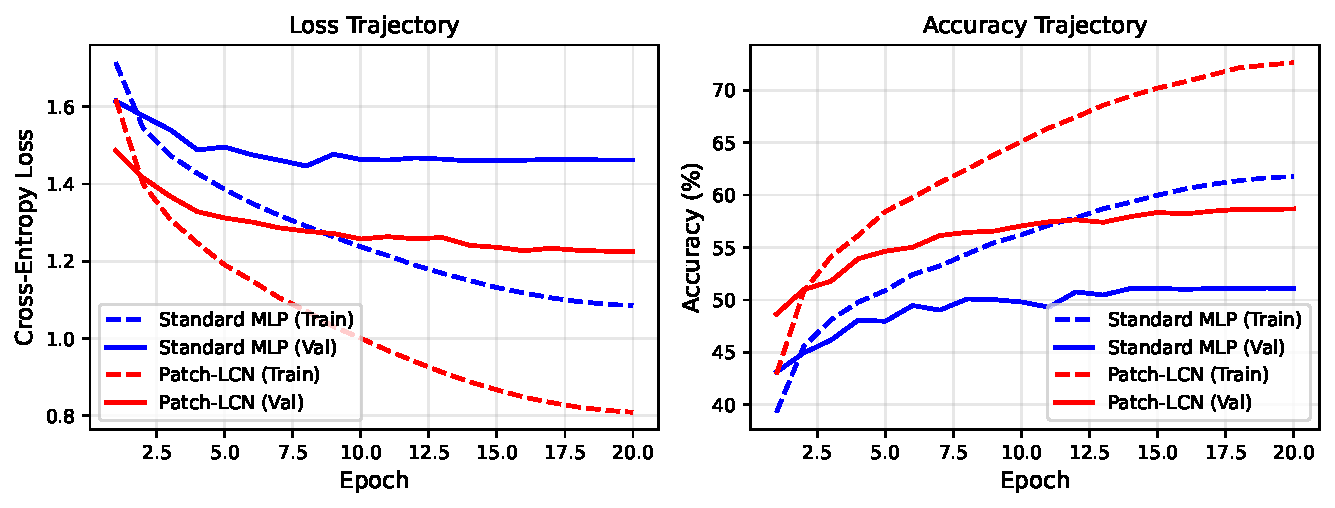
\includegraphics[width=0.78\linewidth]{figures/q1a_learning_curves.pdf}
\caption{Q1(a) Training and validation learning curves for Standard MLP vs. Patch-LCN over 20 epochs.}
\label{fig:q1a}
\end{figure}

\paragraph{Empirical Evidence and Scientific Nuance.}
As shown in Table~\ref{tab:q1a} and Figure~\ref{fig:q1a}, restricting first-layer receptive fields to $8 \times 8$ local spatial neighborhoods yields an immediate $+7.17\%$ test accuracy increase ($50.77\% \to 57.94\%$), even without translational weight sharing. 

However, from an epistemological perspective, we must state the precise scientific boundary of this comparison. Patch-LCN differs from the Standard MLP in two intertwined structural properties:
\begin{enumerate}
    \item \textbf{Local Connectivity Prior:} Pixel interactions are restricted to biologically plausible $8 \times 8$ neighborhoods.
    \item \textbf{Hierarchical Manifold Organization:} In Patch-LCN, the first layer produces $560$ activations ($16 \times 35$), preventing cross-patch linear combinations until the second layer. In the Standard MLP, cross-patch interactions occur immediately across all $3{,}072$ coordinates through a narrower 36-dimensional bottleneck.
\end{enumerate}
Thus, while this experiment conclusively refutes $H_2$ (proving that parameter starvation alone does not explain MLP failure), it isolates local spatial receptive fields jointly with block-structured covariance decoupling.

\subsection{Q1(b): Memorization Dynamics Under Label Noise}
\paragraph{Formulation and Effective Corruption Rate.}
To examine whether high-capacity networks learn genuine generalizable visual features before memorizing arbitrary labels, we deploy a High-Capacity MLP ($3{,}072 \to 512 \to 512 \to 10$, $1{,}841{,}162$ trainable parameters) providing $\sim 41$ parameters per training image.

We introduce label noise by selecting exactly $50\%$ of the training images ($22{,}500$ out of $45{,}000$) uniformly at random without replacement and re-assigning their labels via uniform sampling: $\tilde{y}_i \sim \text{Uniform}(\{0, \dots, 9\})$. 
Crucially, because uniform sampling over $K=10$ classes has a $1/K = 10\%$ probability of re-sampling the ground-truth label, the \textbf{effective label corruption rate} is:
\begin{equation}
    \eta_{\text{eff}} = \eta_{\text{nominal}} \times \left(1 - \frac{1}{K}\right) = 0.50 \times \left(1 - \frac{1}{10}\right) = 0.450 \quad (45.00\%).
\end{equation}
Specifically, exactly $20{,}250$ images ($45.00\%$) had their class labels altered, while $2{,}250$ selected images ($5.00\%$) chanced back to their true class, resulting in $55.00\%$ total clean labels in the training set. The $5{,}000$-sample validation set remained $100\%$ clean.

\begin{figure}[t]
\centering
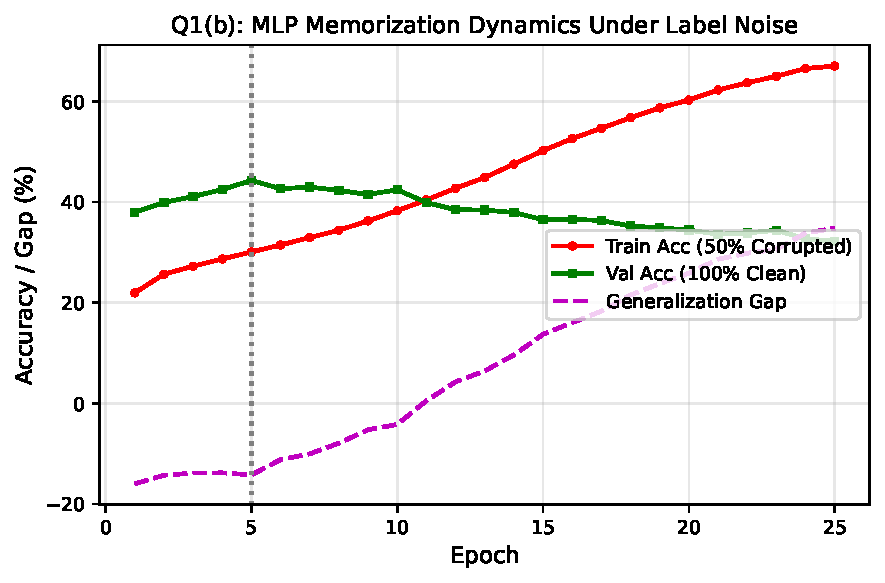
\includegraphics[width=0.78\linewidth]{figures/q1b_memorization_trajectory.pdf}
\caption{Q1(b) Memorization dynamics of High-Capacity MLP under 45\% effective label noise over 25 epochs. Clean validation accuracy peaks at Epoch 5 (44.30\%) before collapsing under active memorization.}
\label{fig:q1b}
\end{figure}

\begin{table}[t]
\centering
\caption{Q1(b) Trajectory checkpoints illustrating the transition from early visual learning to brute-force label fitting.}
\label{tab:q1b}
\resizebox{\columnwidth}{!}{
\begin{tabular}{ccccc}
\toprule
\textbf{Epoch} & \textbf{Train Acc (Noisy)} & \textbf{Val Acc (Clean)} & \textbf{Discrepancy} & \textbf{Phase Regime} \\
\midrule
$1$  & $28.53\%$ & $37.94\%$ & $-9.41\%$ & Coherent Feature Learning \\
$3$  & $35.80\%$ & $41.10\%$ & $-5.30\%$ & Spectral Alignment \\
$\mathbf{5}$  & $\mathbf{39.92\%}$ & $\mathbf{44.30\%}$ & $\mathbf{-4.38\%}$ & \textbf{Peak Generalization} \\
$8$  & $42.11\%$ & $42.30\%$ & $-0.19\%$ & Plateau Transition \\
$11$ & $42.47\%$ & $41.94\%$ & $+0.53\%$ & Trajectory Crossover \\
$15$ & $48.60\%$ & $38.10\%$ & $+10.50\%$ & Active Memorization \\
$20$ & $57.85\%$ & $34.50\%$ & $+23.35\%$ & Label Fitting \\
$25$ & $\mathbf{67.02\%}$ & $\mathbf{32.22\%}$ & $\mathbf{+34.80\%}$ & Overfitting Regime \\
\bottomrule
\end{tabular}
}
\end{table}

\begin{table}[t]
\centering
\caption{Q1(b) Comprehensive multi-subset accuracy audit on the saved checkpoint at Epoch 25 without retraining.}
\label{tab:q1b_audit}
\resizebox{\columnwidth}{!}{
\begin{tabular}{lcc}
\toprule
\textbf{Evaluated Partition / Subset} & \textbf{Sample Count ($N$)} & \textbf{Accuracy} \\
\midrule
1. Unselected Clean Train Subset & $22{,}500$ & $\mathbf{78.60\%}$ \\
2. Corrupted Train (vs. Noisy Assigned Target) & $22{,}500$ & $59.47\%$ \\
3. Corrupted Train (vs. True Ground Truth) & $22{,}500$ & $19.90\%$ \\
4. Clean Validation Set & $5{,}000$ & $32.22\%$ \\
\midrule
\textbf{True In-Distribution Gen Gap} (Row 1 $-$ Row 4) & — & $\mathbf{+46.38\%}$ \\
\textbf{Cross-Distribution Gap} (Row 2 $-$ Row 4) & — & $+27.25\%$ \\
\bottomrule
\end{tabular}
}
\end{table}

\paragraph{Analysis of Spectral Dynamics and Learning Trajectory.}
Tracking the optimization dynamics in Figure~\ref{fig:q1b} and Tables~\ref{tab:q1b} and~\ref{tab:q1b_audit} reveals three distinct phases:
\begin{enumerate}
    \item \textbf{Early Spectral Bias (Epochs 1--5):} Despite $45\%$ of training labels being corrupted, clean validation accuracy rises monotonically from $37.94\%$ to a peak of $\mathbf{44.30\%}$ at Epoch 5. Because true semantic visual patterns are shared across thousands of images, their stochastic gradients constructively align along low-frequency principal components, driving rapid early generalization.
    \item \textbf{Trajectory Crossover (Epoch 11):} At Epoch 11, training accuracy on noisy targets ($42.47\%$) surpasses clean validation accuracy ($41.94\%$), marking the boundary where gradient descent exhausts coherent signal and begins fitting unstructured noise.
    \item \textbf{Brute-Force Memorization (Epochs 12--25):} To fit random label noise, the network must memorize high-frequency sample-specific residuals~\cite{arpit2017closer}. By Epoch 25, training accuracy reaches $67.02\%$, while clean validation accuracy drops by $-12.08\%$ to $32.22\%$.
\end{enumerate}

\paragraph{Multi-Subset Audit and Generalization Gap Semantics.}
A crucial methodological distinction must be drawn regarding the generalization gap. When training on corrupted data, the difference $\text{TrainAcc}_{\text{noisy}} - \text{ValAcc}_{\text{clean}}$ is a \textit{cross-distribution transfer discrepancy} caused by synthetic distribution shift. 

Evaluating the checkpoint on individual subsets (Table~\ref{tab:q1b_audit}) establishes that the model achieves $\mathbf{78.60\%}$ accuracy on uncorrupted training examples and $\mathbf{59.47\%}$ on corrupted training targets, but collapses to $\mathbf{19.90\%}$ when predicting the true class of corrupted samples. The true in-distribution generalization gap on clean data is:
\begin{equation}
    \Delta_{\text{in-dist}} = \text{Acc}(S_{\text{clean\_train}}) - \text{Acc}(\mathcal{D}_{\text{val}}) = 78.60\% - 32.22\% = +46.38\%,
\end{equation}
demonstrating that memorizing $22{,}500$ random labels distorts the representation space, degrading clean feature generalization across all partitions.

\section{Q2: CNN vs. MLP Under Controlled Spatial Disruption}
\label{sec:q2}

\subsection{Q2(a): Baseline Comparison Under Parameter Parity}
\paragraph{FairCNN Architecture.}
To eliminate parameter capacity as a confounding factor when comparing convolutional and fully connected representations, we construct a 4-stage convolutional network, termed \textbf{FairCNN}, designed to precisely match the $\sim 112\text{k}$ parameter budget of the Standard MLP:
\begin{itemize}
    \item \textbf{Stage 1:} $\text{Conv2d}(3 \to 24, k=3, p=1) \to \text{BatchNorm} \to \text{ReLU}$ ($696$ params)
    \item \textbf{Stage 2:} $\text{Conv2d}(24 \to 48, k=3, s=2, p=1) \to \text{BatchNorm} \to \text{ReLU}$ ($10{,}464$ params)
    \item \textbf{Stage 3:} $\text{Conv2d}(48 \to 72, k=3, s=2, p=1) \to \text{BatchNorm} \to \text{ReLU}$ ($31{,}248$ params)
    \item \textbf{Stage 4:} $\text{Conv2d}(72 \to 96, k=3, s=2, p=1) \to \text{BatchNorm} \to \text{ReLU}$ ($62{,}400$ params)
    \item \textbf{Pooling \& Head:} $\text{AdaptiveAvgPool2d}((1, 1)) \to \text{Linear}(96 \to 64) \to \text{ReLU} \to \text{Linear}(64 \to 10)$ ($640 + 6{,}208 + 650 = 7{,}098$ params)
\end{itemize}
Total trainable parameters for FairCNN: $\mathbf{111{,}906}$. This differs from the Standard MLP ($112{,}330$ parameters) by merely $424$ parameters ($\mathbf{0.38\%}$ relative difference).

\paragraph{Clean Baseline Performance.}
Under identical training protocols ($20$ epochs, AdamW $\eta=10^{-3}$, cosine annealing, batch size $64$, seed $26013$), FairCNN achieves a clean test accuracy of $\mathbf{72.05\%}$ compared to the Standard MLP's $\mathbf{50.77\%}$—an absolute advantage of $\mathbf{+21.28\%}$ (Table~\ref{tab:q2_matrix}). This confirms the profound sample efficiency granted by convolutional inductive biases under matched capacity.

\subsection{Q2(b) \& Q2(c): Controlled Spatial Disruptions}
\paragraph{Transform Formulations.}
We design a $2 \times 3$ factorial experiment testing both architectures across three topological conditions:
\begin{enumerate}
    \item \textbf{Clean Condition:} Natural, unperturbed CIFAR-10 images.
    \item \textbf{Pixel-Permuted Condition (Q2b):} A single fixed spatial bijection $\pi: \{1, \dots, 32\} \times \{1, \dots, 32\} \to \{1, \dots, 32\} \times \{1, \dots, 32\}$ generated with seed $26013$ is applied to all channels across all training, validation, and test samples. This destroys 100\% of 2D spatial continuity while preserving exact pixel intensity histograms and marginal color distributions.
    \item \textbf{Patch-Permuted Condition (Q2c):} Each image is decomposed into 16 non-overlapping $8 \times 8$ blocks, and a fixed block permutation $\Pi: \{1, \dots, 16\} \to \{1, \dots, 16\}$ is applied. Intra-patch spatial smoothness and edge gradients are 100\% preserved, but global semantic spatial layout is scrambled.
\end{enumerate}

\begin{table*}[t]
\centering
\caption{Q2 Factorial Matrix: Impact of Spatial Structure Disruption on FairCNN vs. Standard MLP ($\sim 112\text{k}$ parameters). Evaluated on the official CIFAR-10 test set ($N=10{,}000$), reporting test accuracy, mean confidence, confidence on correct/incorrect subsets, and Expected Calibration Error (ECE, $M=15$ bins).}
\label{tab:q2_matrix}
\small
\begin{tabular}{llcccccc}
\toprule
\textbf{Architecture} & \textbf{Spatial Condition} & \textbf{Parameters} & \textbf{Test Acc} & \textbf{Mean Conf} & \textbf{Conf (Corr)} & \textbf{Conf (Incorr)} & \textbf{ECE} \\
\midrule
\textbf{FairCNN} & Clean Baseline          & $111{,}906$ & $\mathbf{72.05\%}$ & $0.833$ & $0.890$ & $0.689$ & $0.1141$ \\
\textbf{FairCNN} & Patch-Permuted ($8\times 8$) & $111{,}906$ & $65.56\%$ & $0.793$ & $0.858$ & $0.668$ & $0.1371$ \\
\textbf{FairCNN} & Pixel-Permuted          & $111{,}906$ & $53.89\%$ & $0.599$ & $0.681$ & $0.504$ & $0.0612$ \\
\midrule
\textbf{Standard MLP} & Clean Baseline     & $112{,}330$ & $50.77\%$ & $0.575$ & $0.659$ & $0.489$ & $0.0675$ \\
\textbf{Standard MLP} & Patch-Permuted ($8\times 8$) & $112{,}330$ & $50.17\%$ & $0.572$ & $0.658$ & $0.485$ & $0.0700$ \\
\textbf{Standard MLP} & Pixel-Permuted     & $112{,}330$ & $50.55\%$ & $0.580$ & $0.667$ & $0.491$ & $0.0744$ \\
\bottomrule
\end{tabular}
\end{table*}

\begin{figure}[t]
\centering
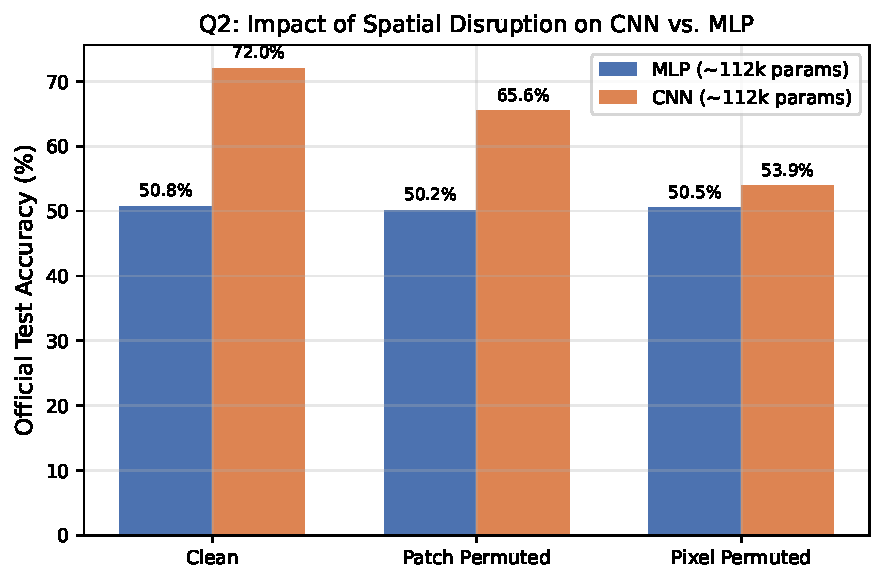
\includegraphics[width=0.78\linewidth]{figures/q2_spatial_disturbance.pdf}
\caption{Q2 Official test accuracy across Clean, Patch-Permuted, and Pixel-Permuted CIFAR-10 for FairCNN vs. Standard MLP.}
\label{fig:q2_bar}
\end{figure}

\begin{figure}[t]
\centering
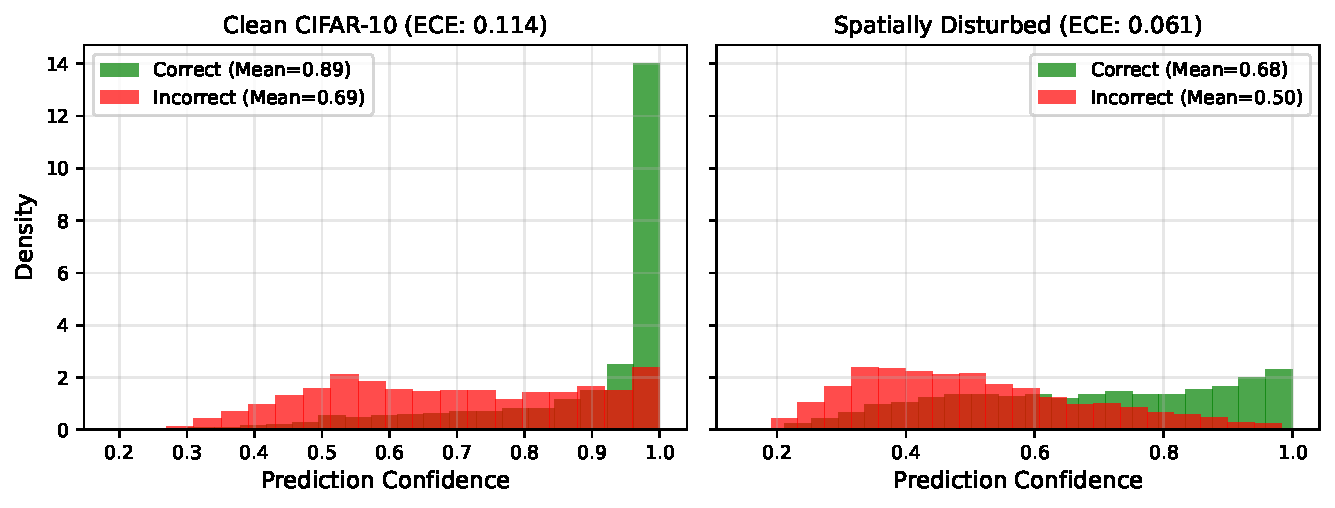
\includegraphics[width=0.78\linewidth]{figures/q2c_confidence_analysis.pdf}
\caption{Q2 Prediction confidence density distributions for correct vs. incorrect classifications on Clean vs. Spatially Disturbed inputs.}
\label{fig:q2_conf}
\end{figure}

\subsection{Theoretical and Empirical Analysis}
\paragraph{Complete Spatial Permutation Invariance of MLPs.}
As documented in Table~\ref{tab:q2_matrix} and Figure~\ref{fig:q2_bar}, the Standard MLP exhibits virtually identical test performance across all three conditions:
\begin{equation}
    \text{Acc}_{\text{clean}} = 50.77\%, \quad \text{Acc}_{\text{patch}} = 50.17\%, \quad \text{Acc}_{\text{pixel}} = 50.55\%.
\end{equation}
The variation across all conditions is within $\pm 0.30\%$ (standard stochastic training noise). 
\textit{Proof of Invariance:} For any linear transformation $\mathbf{y} = \mathbf{W}\mathbf{x}$ and any orthogonal permutation matrix $\mathbf{P}$, substituting permuted input $\tilde{\mathbf{x}} = \mathbf{P}\mathbf{x}$ yields $\mathbf{y} = \mathbf{W}\mathbf{P}\mathbf{x} = \tilde{\mathbf{W}}\mathbf{x}$. Because fully connected weight initializations are drawn from isotropic distributions (e.g., Kaiming normal), the optimization dynamics are isomorphic under any fixed coordinate permutation. The MLP possesses exactly zero spatial inductive bias.

\paragraph{Hierarchical Breakdown of Convolutional Inductive Biases.}
In stark contrast, FairCNN displays dramatic sensitivity to spatial topology:
\begin{enumerate}
    \item \textbf{Patch Permutation (Preserving Local Features):} When $8 \times 8$ blocks are shuffled, CNN accuracy drops by only $-6.49\%$ ($72.05\% \to 65.56\%$). Because local receptive fields in early convolutional stages remain unperturbed, low-level edge detectors and textural filters fire normally. Performance degrades solely because deeper pooling layers cannot assemble these local parts into coherent global canonical silhouettes.
    \item \textbf{Pixel Permutation (Destruction of Locality):} When individual pixels are shuffled, CNN accuracy collapses by $-18.16\%$ ($72.05\% \to 53.89\%$). Local receptive fields now sample uncorrelated pixels across disparate regions of the visual field.
    \item \textbf{Why Pixel-Permuted CNN Outperforms MLP ($53.89\%$ vs. $50.55\%$):} Even under complete spatial scrambling, the CNN retains a $+3.34\%$ advantage over the MLP. This occurs because convolutional weight sharing forces parameter tying across all grid locations, acting as a strong structural regularizer that reduces parameter count and bounds estimation variance.
\end{enumerate}

\subsection{Uncertainty and Calibration Dynamics (ECE)}
To assess model reliability under spatial degradation, we evaluate the Maximum Softmax Probability (confidence) and Expected Calibration Error (ECE) with $M=15$ bins:
\begin{equation}
    \text{ECE} = \sum_{m=1}^M \frac{|B_m|}{N} \left| \text{acc}(B_m) - \text{conf}(B_m) \right|.
\end{equation}
As shown in Table~\ref{tab:q2_matrix} and Figure~\ref{fig:q2_conf}:
\begin{itemize}
    \item \textbf{Clean CNN Overconfidence:} On clean data, the CNN displays classical deep overconfidence~\cite{guo2017calibration} ($\text{ECE} = 0.1141$, mean confidence $83.3\%$ vs. accuracy $72.1\%$). Even on misclassified samples, average confidence remains high ($0.689$).
    \item \textbf{Patch-Permuted Peak Miscalibration:} Patch permutation produces the highest calibration error ($\text{ECE} = 0.1371$). The CNN retains high internal confidence from valid local patch activations ($0.793$), but errors increase sharply due to global structural incoherence.
    \item \textbf{Pixel-Permuted Softmax Flattening:} Under pixel permutation, CNN confidence drops sharply ($0.833 \to 0.599$). Because inputs resemble unstructured noise, logits disperse, reducing overconfidence and artificially lowering ECE to $0.0612$.
    \item \textbf{MLP Calibration Stability:} Across all three conditions, MLP confidence remains conservative ($0.57-0.58$) with ECE between $0.067$ and $0.074$, reflecting low capacity and diffuse posterior distributions.
\end{itemize}

\section{Q3: Convolutional Autoencoders and Representation Probing}
\label{sec:q3}

\subsection{Q3(a): Bottleneck Capacity Sweep and Model Selection}
\paragraph{Symmetrical Convolutional Architecture.}
To investigate unsupervised representation learning, we design a symmetrical convolutional autoencoder where the encoder progressively downsamples the image from $32 \times 32$ to $2 \times 2$ via stride-2 convolutions, followed by a linear projection into bottleneck dimension $d \in \{64, 256, 1024\}$:
\begin{itemize}
    \item \textbf{Encoder:} $\text{Conv}(3 \to 32) \to \text{Conv}(32 \to 48) \to \text{Conv}(48 \to 64) \to \text{Conv}(64 \to 64) \to \text{Flatten} (256\text{-D}) \to \text{Linear}(256 \to d)$.
    \item \textbf{Decoder:} $\text{Linear}(d \to 256) \to \text{Reshape} (64 \times 2 \times 2) \to \text{Deconv}(64 \to 64) \to \text{Deconv}(64 \to 48) \to \text{Deconv}(48 \to 32) \to \text{Deconv}(32 \to 3) \to \text{Sigmoid}$.
\end{itemize}
Outputs are bounded in $[0, 1]$ via Sigmoid to match unit-normalized input images. Training optimizes Mean Squared Error (MSE) loss for $20$ epochs using AdamW ($\eta=10^{-3}$, cosine annealing, batch size $64$, seed $26013$).

\begin{table}[t]
\centering
\caption{Q3(a) Convolutional Autoencoder parameter counts and reconstruction MSE across bottleneck capacities $d \in \{64, 256, 1024\}$. Model selection conducted strictly on the $5{,}000$-sample validation set.}
\label{tab:q3a_mse}
\resizebox{\columnwidth}{!}{
\begin{tabular}{lccccc}
\toprule
\textbf{Bottleneck $d$} & \textbf{Enc Params} & \textbf{Dec Params} & \textbf{Total Params} & \textbf{Val MSE} & \textbf{Test MSE} \\
\midrule
$d = 64$   & $95{,}856$  & $95{,}987$  & $191{,}843$ & $0.008134$ & $0.008159$ \\
$d = 256$  & $145{,}200$ & $145{,}139$ & $290{,}339$ & $0.006373$ & $0.006409$ \\
$\mathbf{d = 1024}$ & $\mathbf{342{,}576}$ & $\mathbf{341{,}747}$ & $\mathbf{684{,}323}$ & $\mathbf{0.005855}$ & $\mathbf{0.005888}$ \\
\midrule
\textbf{DAE ($b=256$)} & $145{,}200$ & $145{,}139$ & $290{,}339$ & $0.007734$ & $0.007760$ \\
\bottomrule
\end{tabular}
}
\end{table}

\begin{figure}[t]
\centering
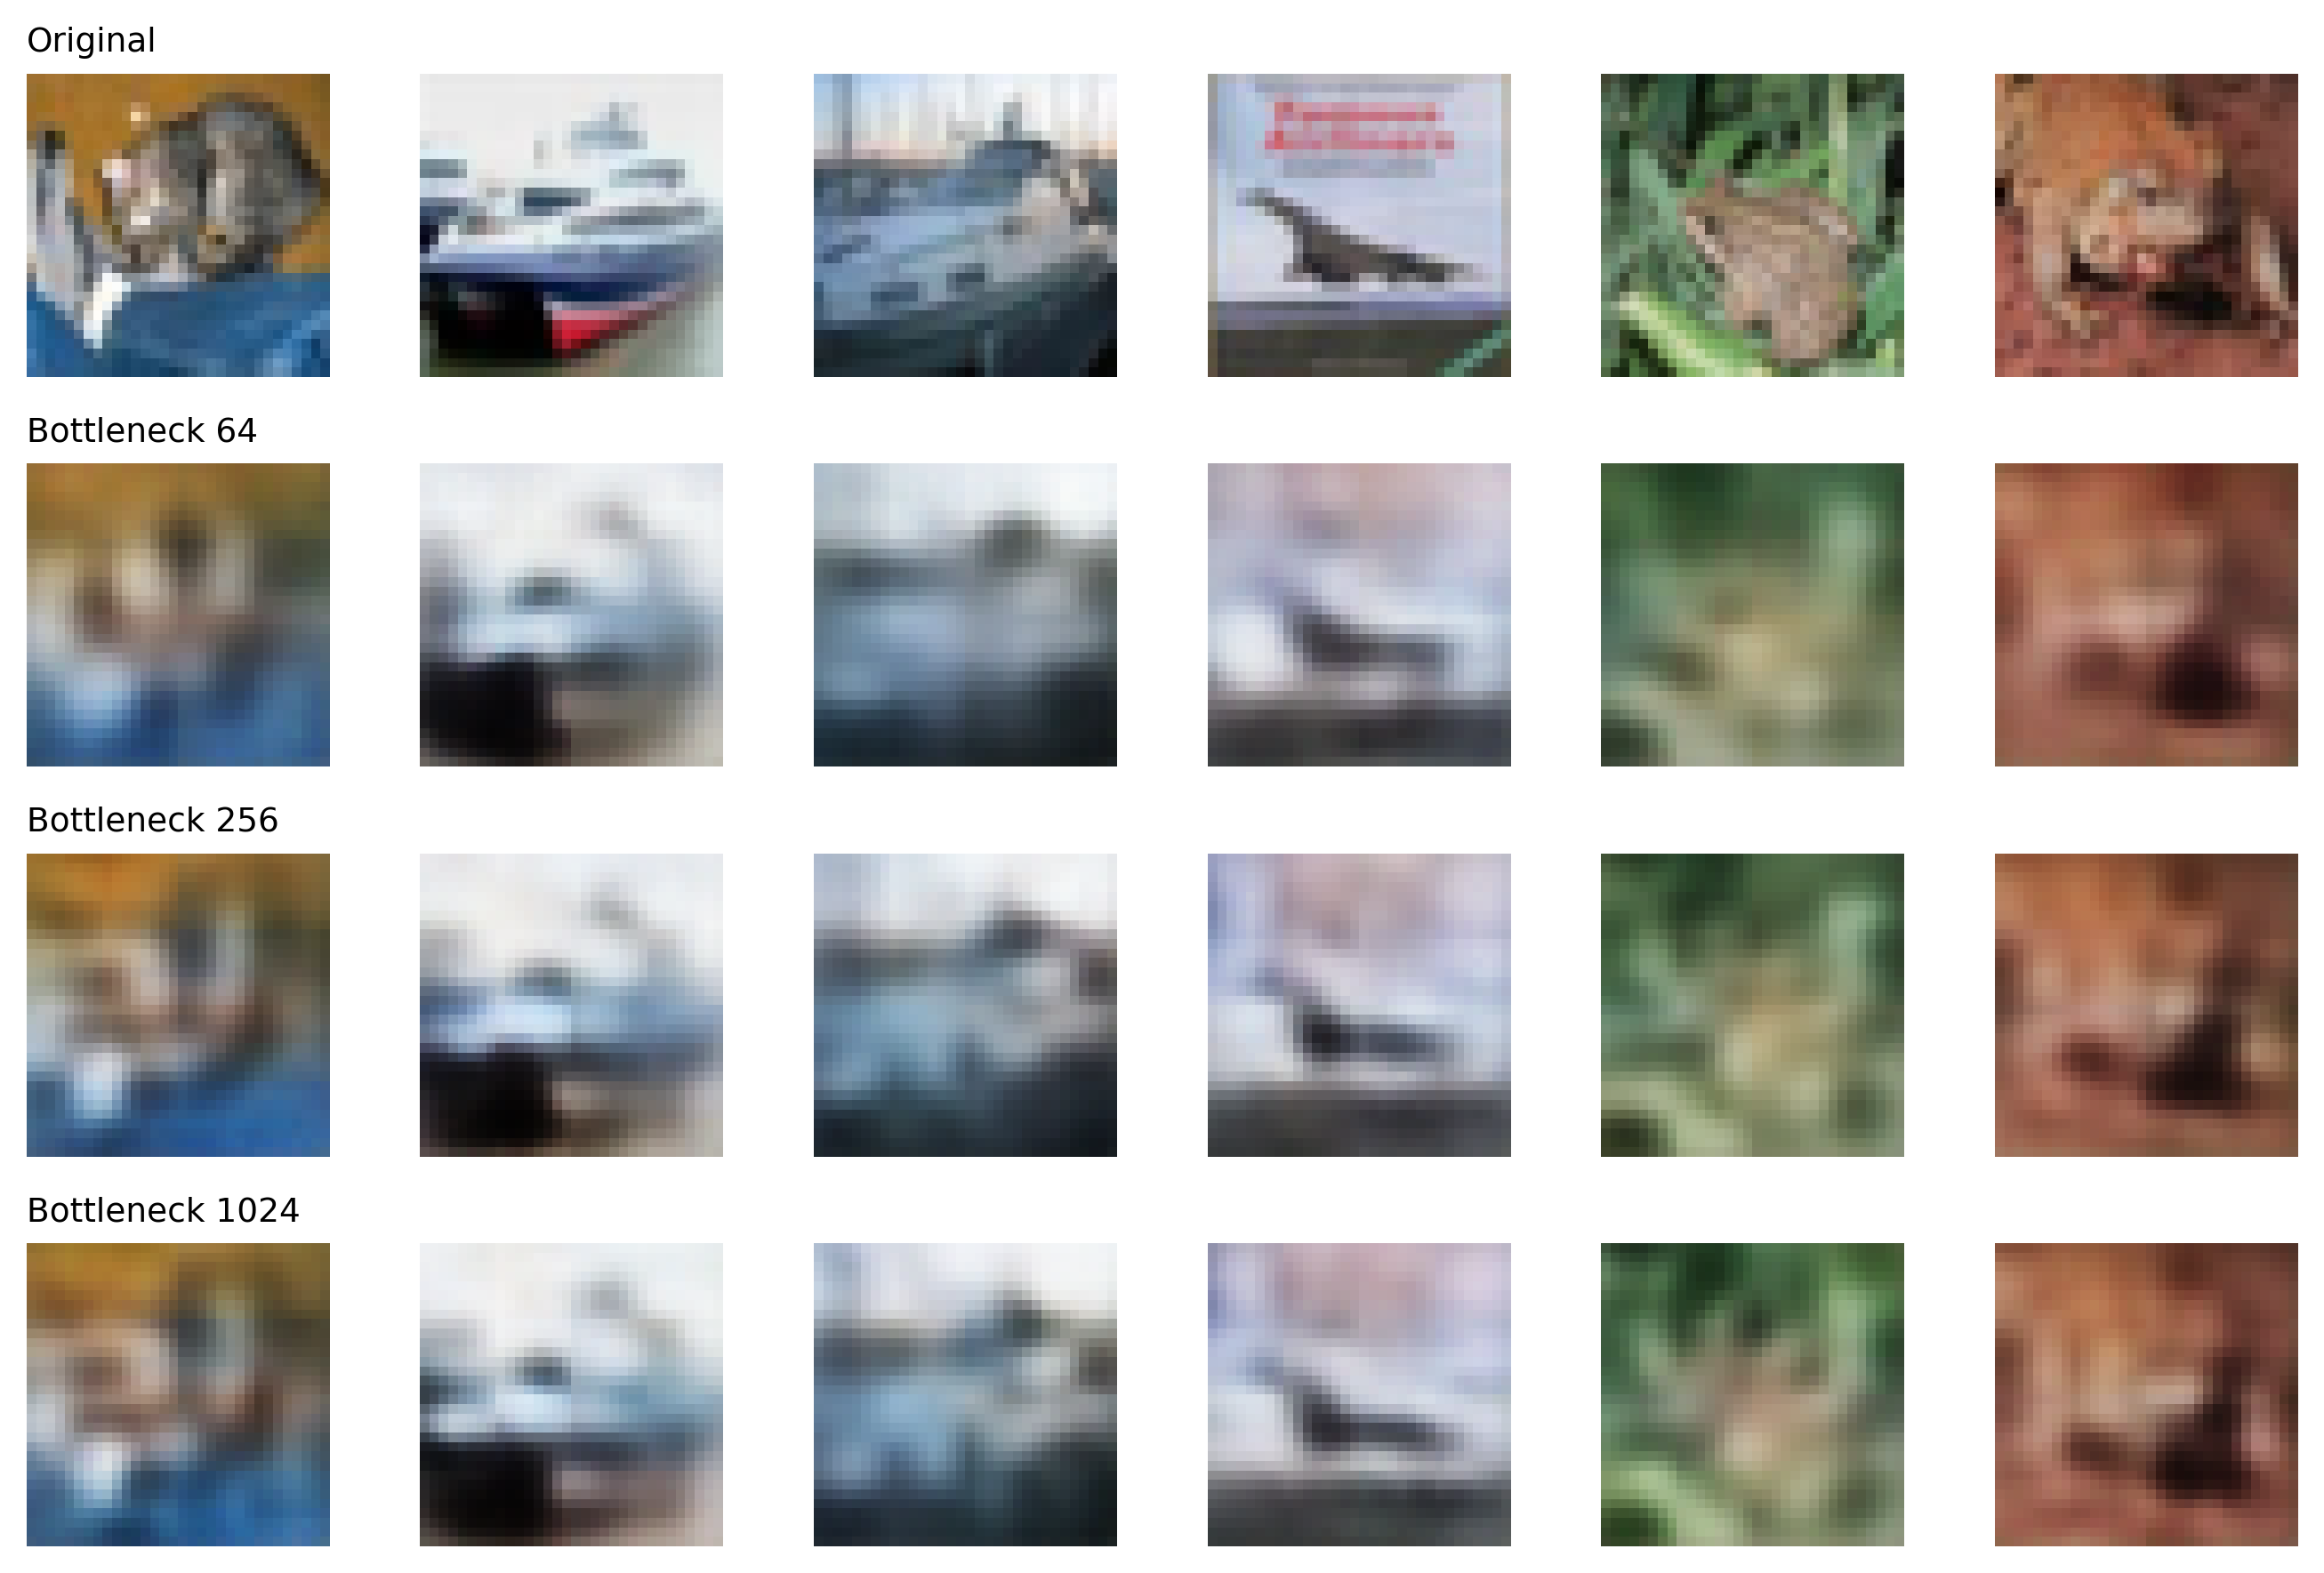
\includegraphics[width=0.78\linewidth]{figures/q3a_reconstruction_grid.png}
\caption{Q3(a) Test image reconstructions across bottleneck capacities $d \in \{64, 256, 1024\}$ compared against original CIFAR-10 inputs.}
\label{fig:q3a_grid}
\end{figure}

\paragraph{Validation-Based Model Selection.}
As required by the experimental integrity protocol, the clean autoencoder was selected strictly using validation reconstruction error (Table~\ref{tab:q3a_mse}):
\begin{equation}
\begin{aligned}
    \text{Val MSE}(1024) &= 0.005855 < 0.006373 \, (b=256) \\
    &< 0.008134 \, (b=64).
\end{aligned}
\end{equation}
Bottleneck $\mathbf{d = 1024}$ was formally selected. The official test set was evaluated strictly post-selection, yielding $\text{Test MSE} = 0.005888$. 

As visualized in Figure~\ref{fig:q3a_grid}, expanding bottleneck capacity allows the network to reconstruct high-frequency texture details and object boundaries that are blurred under $d=64$.

\subsection{Q3(b): Denoising Autoencoder \& Downstream Recovery}
\paragraph{Denoising Protocol.}
We construct a Denoising Autoencoder (DAE) with $b=256$ trained with zero class supervision. The encoder receives corrupted inputs $\tilde{\mathbf{x}} = \text{clip}(\mathbf{x} + \boldsymbol{\epsilon}, 0, 1)$, where $\boldsymbol{\epsilon} \sim \mathcal{N}(\mathbf{0}, \sigma^2 \mathbf{I})$ with $\sigma = 0.2$, while the reconstruction loss is computed strictly against the uncorrupted target image $\mathbf{x}$. The DAE achieves a validation MSE of $0.007734$ and test MSE of $0.007760$.

\begin{figure}[t]
\centering
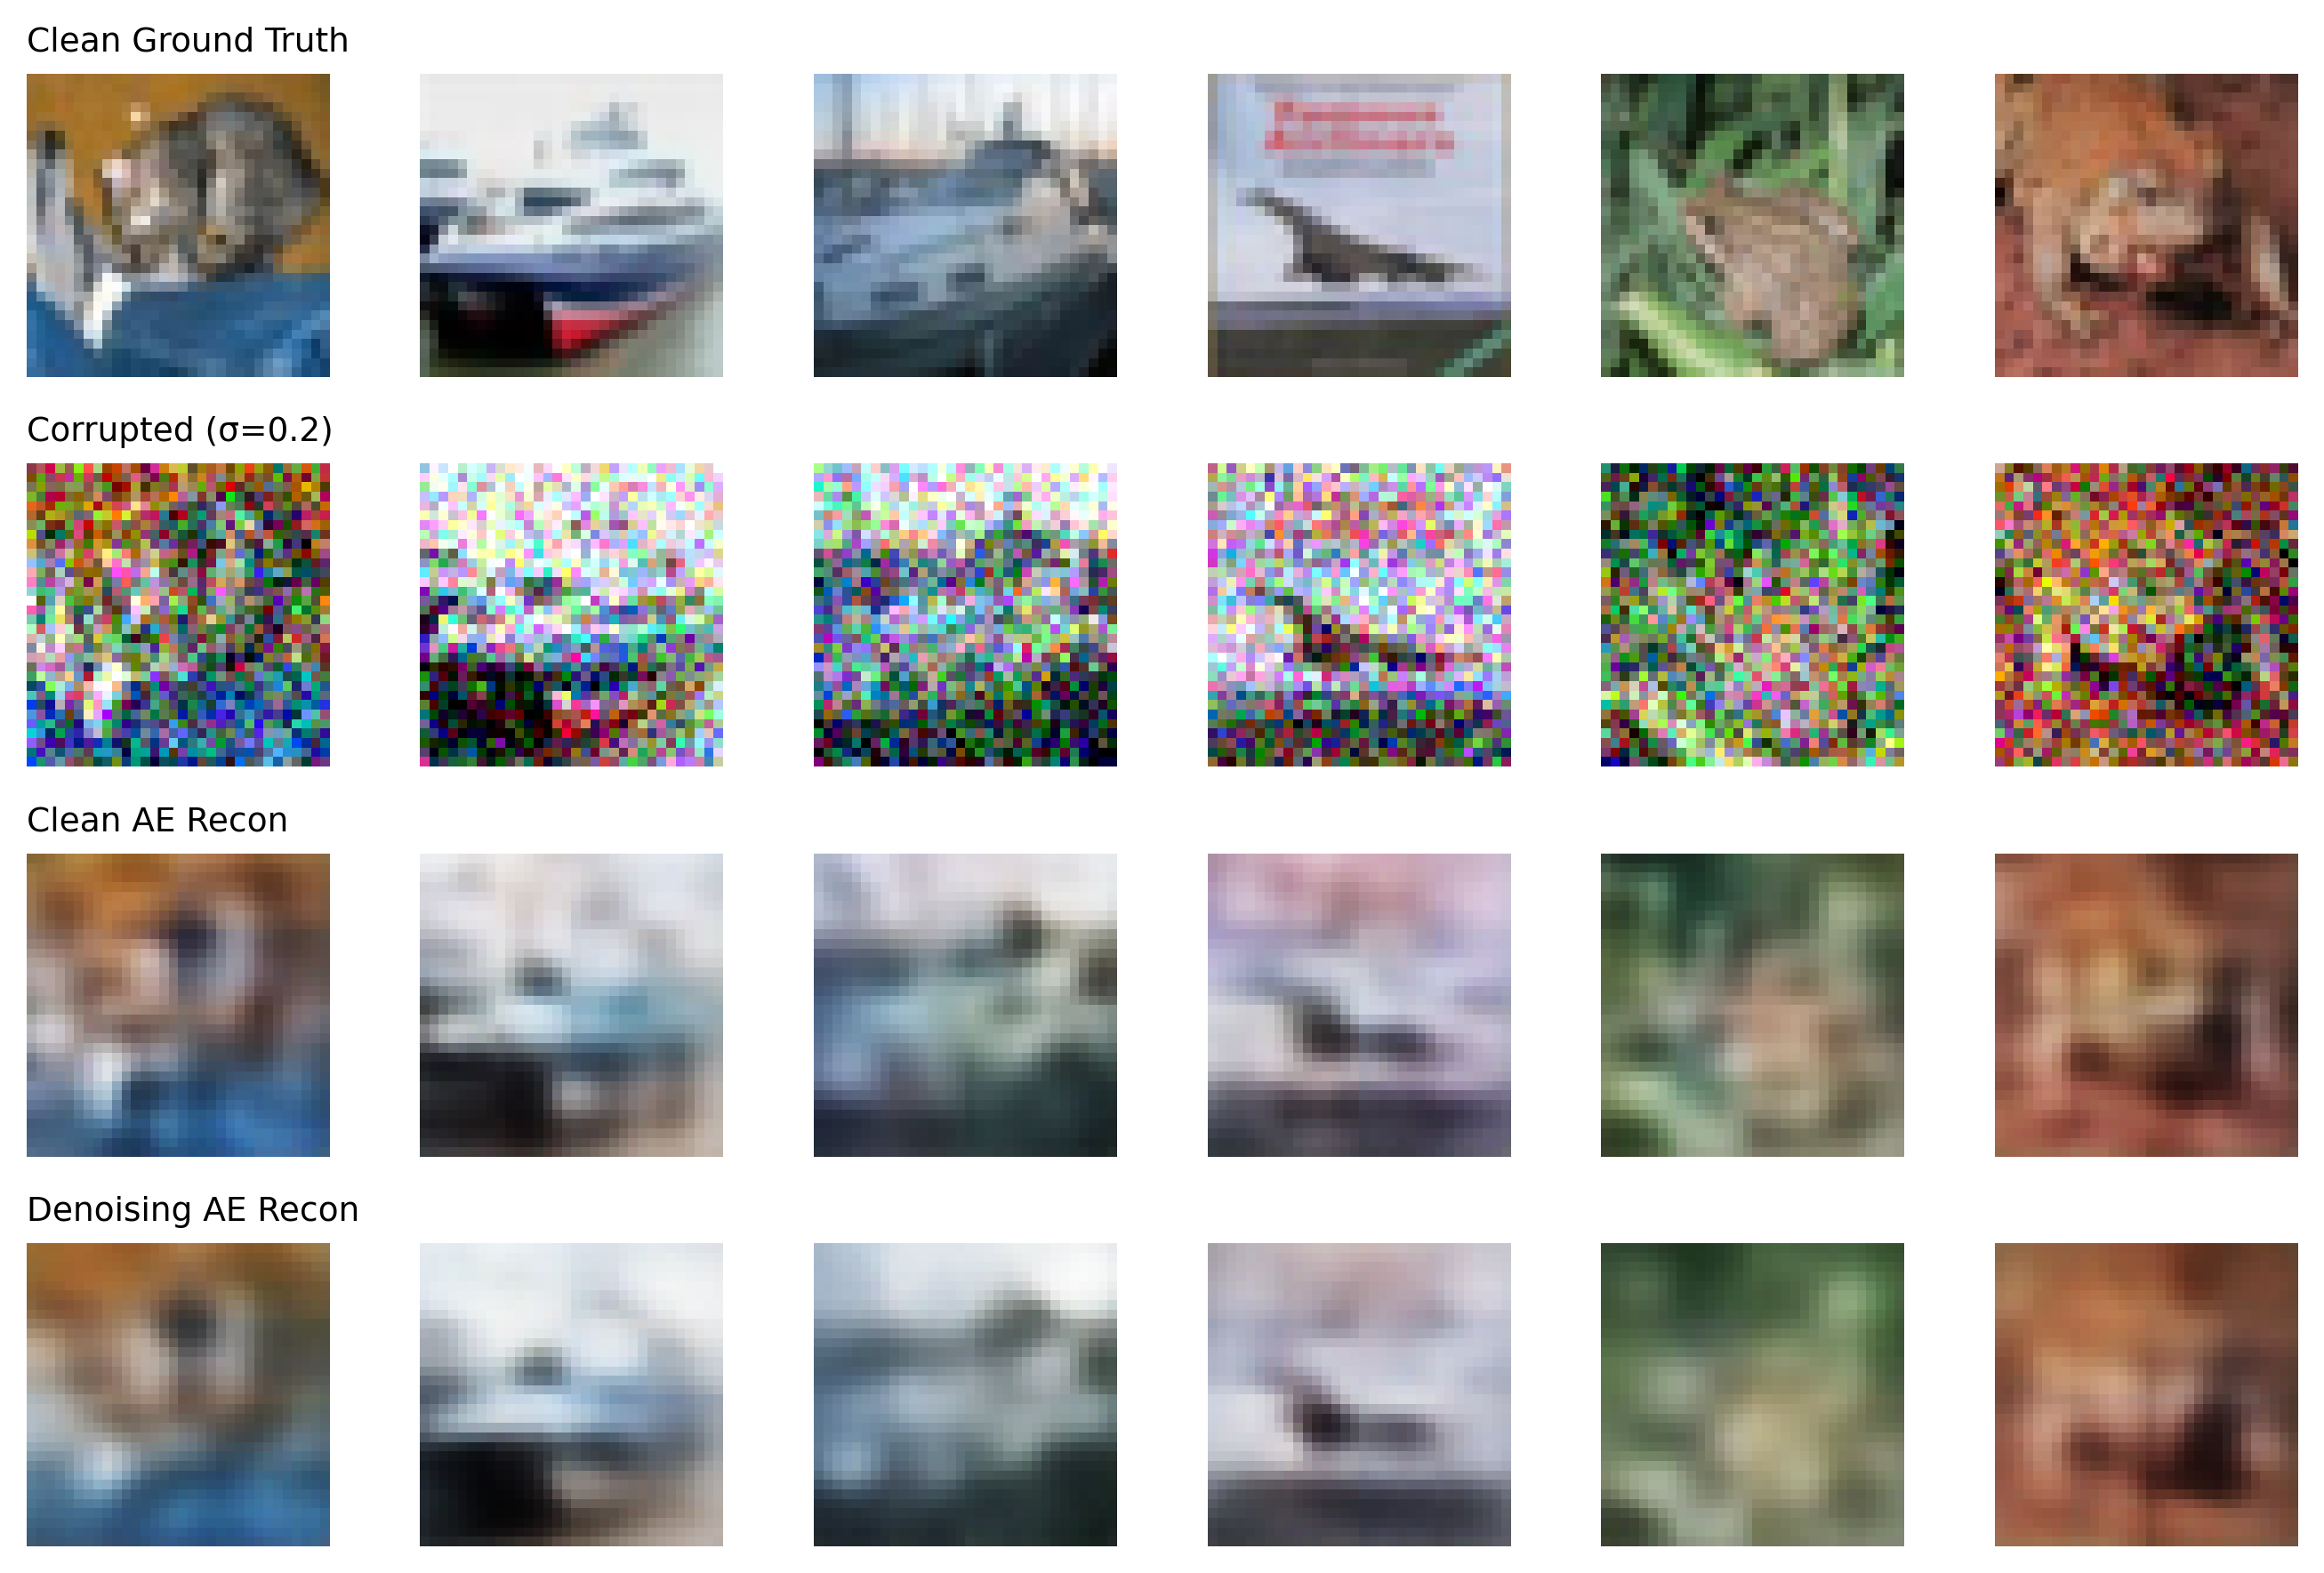
\includegraphics[width=0.78\linewidth]{figures/q3b_denoising_comparison.png}
\caption{Q3(b) Semantic denoising comparison: (Row 1) Clean Ground Truth, (Row 2) Corrupted with $\sigma=0.2$, (Row 3) Clean AE Recon ($b=1024$), (Row 4) DAE Recon ($b=256$).}
\label{fig:q3b_denoise}
\end{figure}

\begin{table}[t]
\centering
\caption{Q3(b) Downstream classification accuracy on the official CIFAR-10 test set using the fixed, frozen FairCNN classifier from Q2(a) ($72.05\%$ clean baseline). Both autoencoders receive identical corrupted test inputs.}
\label{tab:q3b_downstream}
\resizebox{\columnwidth}{!}{
\begin{tabular}{lcc}
\toprule
\textbf{Input Evaluated by Fixed FairCNN} & \textbf{Test Accuracy} & \textbf{Delta vs. Corrupted} \\
\midrule
1. Clean Test Images (Baseline)           & $\mathbf{72.05\%}$ & — \\
2. Corrupted Test Images ($\sigma = 0.2$) Directly & $20.07\%$ & Baseline ($-51.98\%$) \\
3. Clean AE Reconstructions ($b=1024$)    & $27.65\%$ & $\mathbf{+7.58\%}$ \\
4. Denoising AE Reconstructions ($b=256$) & $27.57\%$ & $\mathbf{+7.50\%}$ \\
\bottomrule
\end{tabular}
}
\end{table}

\paragraph{Fixed Downstream Classifier Evaluation.}
To assess whether pixel-level denoising restores semantic utility, we evaluate the reconstructed test images using our fixed, previously trained FairCNN classifier from Q2(a) without retraining or fine-tuning (Table~\ref{tab:q3b_downstream}). 
\begin{enumerate}
    \item \textbf{Susceptibility to Noise:} Directly corrupting images with $\sigma=0.2$ drops CNN classification accuracy from $72.05\%$ to $20.07\%$ (a $-51.98\%$ collapse).
    \item \textbf{Denoising Gain:} Passing corrupted images through either the Clean AE ($27.65\%$) or DAE ($27.57\%$) recovers approximately $+7.5\%$ accuracy over raw corrupted inputs.
    \item \textbf{The Reconstruction Domain Shift:} Despite effective visual smoothing (Figure~\ref{fig:q3b_denoise}), neither autoencoder recovers the clean $72.05\%$ baseline. This exposes a fundamental limitation of unsupervised $L_2$ pixel reconstruction: autoencoders minimize average squared error across all pixels, attenuating sharp edge gradients and high-frequency textures that deep CNN classifiers rely upon for discrimination.
\end{enumerate}

\subsection{Q3(c): Representation Quality vs. Class Information}
\paragraph{Linear Probing Protocol.}
To evaluate the semantic quality of learned representations without fine-tuning, we freeze all encoder weights $\boldsymbol{\theta}_{\text{enc}}^*$ and train a single linear classification layer $\mathbf{y} = \mathbf{W}\mathbf{z} + \mathbf{b}$ on the extracted bottleneck features. Feature standardization $(\boldsymbol{\mu}, \boldsymbol{\sigma})$ is fitted exclusively on training representations. Optimal learning rates and early stopping are determined strictly on validation representations before single test evaluation.

\begin{figure}[t]
\centering
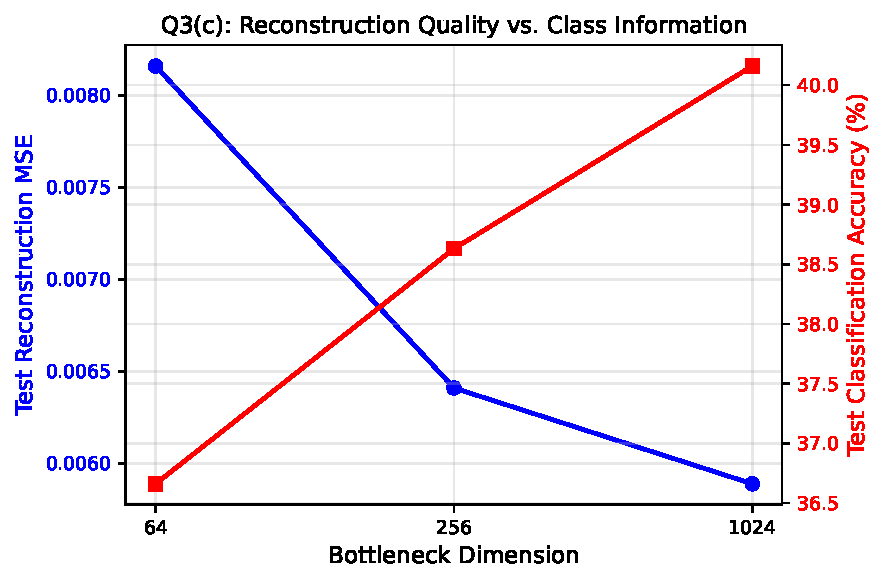
\includegraphics[width=0.78\linewidth]{figures/q3c_reconstruction_vs_class_info.pdf}
\caption{Q3(c) Dual-axis trade-off curve: Test Reconstruction MSE (blue, lower is better) vs. Frozen Linear Probe Test Accuracy (red, higher is better) across bottleneck capacities $d \in \{64, 256, 1024\}$.}
\label{fig:q3c_tradeoff}
\end{figure}

\begin{table}[t]
\centering
\caption{Q3(c) Frozen linear probe classification accuracy and test reconstruction MSE across autoencoder bottlenecks.}
\label{tab:q3c_probe}
\resizebox{\columnwidth}{!}{
\begin{tabular}{lcccc}
\toprule
\textbf{Feature Backbone} & \textbf{Bottleneck $d$} & \textbf{Test MSE} & \textbf{Probe Val Acc} & \textbf{Probe Test Acc} \\
\midrule
Clean AE  & $64$   & $0.008159$ & $36.28\%$ & $36.66\%$ \\
Clean AE  & $256$  & $0.006409$ & $39.32\%$ & $38.63\%$ \\
Clean AE  & $1024$ & $\mathbf{0.005888}$ & $\mathbf{40.16\%}$ & $\mathbf{40.16\%}$ \\
\midrule
DAE       & $256$  & $0.007760$ & $39.30\%$ & $38.77\%$ \\
\bottomrule
\end{tabular}
}
\end{table}

\paragraph{Analysis of Reconstruction vs. Class Information.}
As illustrated in Figure~\ref{fig:q3c_tradeoff} and Table~\ref{tab:q3c_probe}:
\begin{itemize}
    \item \textbf{Monotonic Correlation:} Across clean autoencoders, reconstruction MSE and linear probe accuracy are monotonically aligned: as $d$ expands from $64 \to 1024$, reconstruction error drops from $0.00816 \to 0.00589$, while linear probe test accuracy increases from $36.66\% \to 40.16\%$. A wider bottleneck retains more linearly separable class variance.
    \item \textbf{DAE Compactness:} Notably, the DAE ($b=256$) achieves $38.77\%$ probe accuracy—slightly outperforming the clean AE of identical dimension ($38.63\%$) despite exhibiting higher reconstruction MSE ($0.00776$ vs. $0.00641$). Denoising forces the encoder to discard independent pixel noise, yielding a more robust semantic subspace.
    \item \textbf{The Linear Separability Gap:} Even at $d=1024$, linear probe accuracy reaches only $40.16\%$, far below end-to-end FairCNN ($72.05\%$). Unsupervised reconstruction allocates representational capacity equally to background pixels and foreground objects, proving that pixel-level reconstruction fidelity is insufficient for high-level semantic categorization.
\end{itemize}

\section{Q4 Bonus: Kernel SVMs, Margin Geometry, and Clustering}
\label{sec:q4}

\subsection{Q4(a): Systematic SVM Parameter and Kernel Sweep}
\paragraph{Experimental Protocol and Representation Space.}
To evaluate kernel methods on deep representations, we utilize the frozen 64-dimensional penultimate representation extracted from our trained FairCNN model from Q2(a) (verified at $\mathbf{72.05\%}$ test accuracy). We use the fixed, stratified $5{,}000$-sample training subset $\mathcal{D}_{\text{svm}}$ ($500$ samples per class). Preprocessing via \texttt{StandardScaler} is fitted strictly on the $5{,}000$ training representations and applied frozen to the validation and test splits.

We execute an exhaustive $15$-configuration grid sweep spanning three kernel families and five regularization parameters:
\begin{equation}
\begin{aligned}
    \mathcal{K} &\in \{\text{Linear}, \text{RBF}, \text{Poly} (d=3)\}, \\
    C &\in \{0.01, 0.1, 1.0, 10.0, 100.0\}.
\end{aligned}
\end{equation}

\begin{table}[t]
\centering
\caption{Q4(a) Exhaustive 15-Configuration SVM Grid Sweep on 64-D FairCNN representations. Model selection was conducted strictly using validation accuracy on the full $5{,}000$-sample validation set.}
\label{tab:q4a_sweep}
\resizebox{\columnwidth}{!}{
\begin{tabular}{lccccc}
\toprule
\textbf{Kernel} & \textbf{Reg. $C$} & \textbf{Train Acc} & \textbf{Val Acc ($N=5\text{k}$)} & \textbf{SVs ($N_{\text{SV}}$)} & \textbf{SV Frac ($\rho_{\text{SV}}$)} \\
\midrule
Linear & $0.01$  & $95.32\%$ & $72.84\%$ & $2{,}018$ & $40.36\%$ \\
Linear & $0.1$   & $95.76\%$ & $72.18\%$ & $1{,}118$ & $22.36\%$ \\
Linear & $1.0$   & $96.88\%$ & $71.50\%$ & $875$     & $17.50\%$ \\
Linear & $10.0$  & $97.80\%$ & $70.54\%$ & $854$     & $17.08\%$ \\
Linear & $100.0$ & $98.52\%$ & $69.98\%$ & $844$     & $16.88\%$ \\
\midrule
RBF    & $0.01$  & $91.40\%$ & $72.22\%$ & $4{,}828$ & $96.56\%$ \\
\textbf{RBF} & $\mathbf{0.1}$ & $\mathbf{94.74\%}$ & $\mathbf{72.88\%}$ & $\mathbf{3{,}124}$ & $\mathbf{62.48\%}$ \\
RBF    & $1.0$   & $96.28\%$ & $72.52\%$ & $1{,}788$ & $35.76\%$ \\
RBF    & $10.0$  & $98.32\%$ & $71.92\%$ & $1{,}343$ & $26.86\%$ \\
RBF    & $100.0$ & $99.90\%$ & $71.76\%$ & $1{,}374$ & $27.48\%$ \\
\midrule
Poly ($d=3$) & $0.01$  & $62.32\%$ & $52.38\%$ & $4{,}324$ & $86.48\%$ \\
Poly ($d=3$) & $0.1$   & $84.54\%$ & $67.02\%$ & $2{,}983$ & $59.66\%$ \\
Poly ($d=3$) & $1.0$   & $93.36\%$ & $71.18\%$ & $1{,}840$ & $36.80\%$ \\
Poly ($d=3$) & $10.0$  & $97.26\%$ & $71.42\%$ & $1219$    & $24.38\%$ \\
Poly ($d=3$) & $100.0$ & $99.48\%$ & $70.58\%$ & $1141$    & $22.82\%$ \\
\bottomrule
\end{tabular}
}
\end{table}

\begin{figure}[t]
\centering
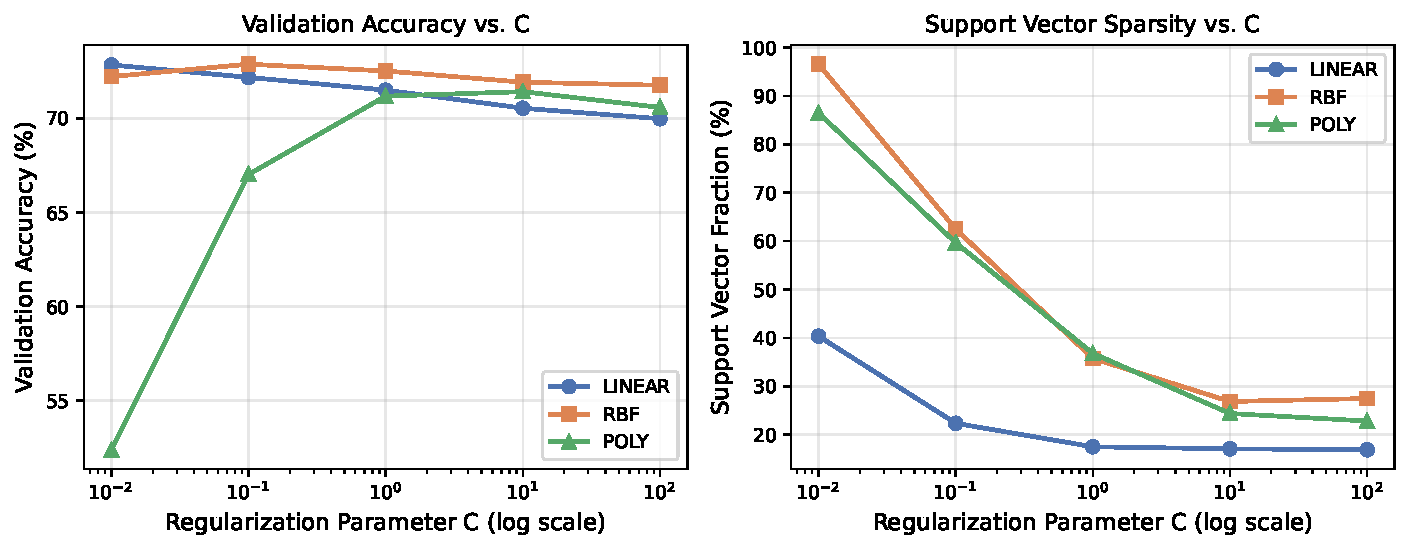
\includegraphics[width=0.78\linewidth]{figures/q4a_svm_sweep.pdf}
\caption{Q4(a) Validation accuracy (left) and support vector fraction (right) as a function of regularization parameter $C$ across Linear, RBF, and Polynomial kernels.}
\label{fig:q4a_sweep}
\end{figure}

\paragraph{Validation-Based Model Selection and Test Result.}
As documented in Table~\ref{tab:q4a_sweep} and Figure~\ref{fig:q4a_sweep}, the **RBF Kernel with $C = 0.1$** achieved the highest accuracy on the full $5{,}000$-sample validation set ($\mathbf{72.88\%}$), with a support vector fraction of $\rho_{\text{SV}} = 62.48\%$ ($3{,}124$ SVs). 

At lower regularization ($C=0.01$), the RBF margin is overly soft, causing nearly all samples to act as support vectors ($\rho_{\text{SV}} = 96.56\%$). At higher regularization ($C \ge 1.0$), the dual solver penalizes margin violations severely, driving training accuracy to $99.90\%$ but inducing validation degradation ($71.76\%$). 

Following selection, the locked model was evaluated strictly once on the official test set:
\begin{equation}
    \text{Official Test Accuracy} = \mathbf{71.64\%}.
\end{equation}
Remarkably, an RBF SVM trained on only $5{,}000$ samples over frozen 64-D CNN features achieves $71.64\%$ accuracy—matching the full end-to-end FairCNN classifier ($72.05\%$) within $0.41\%$.

\begin{figure*}[t]
\centering
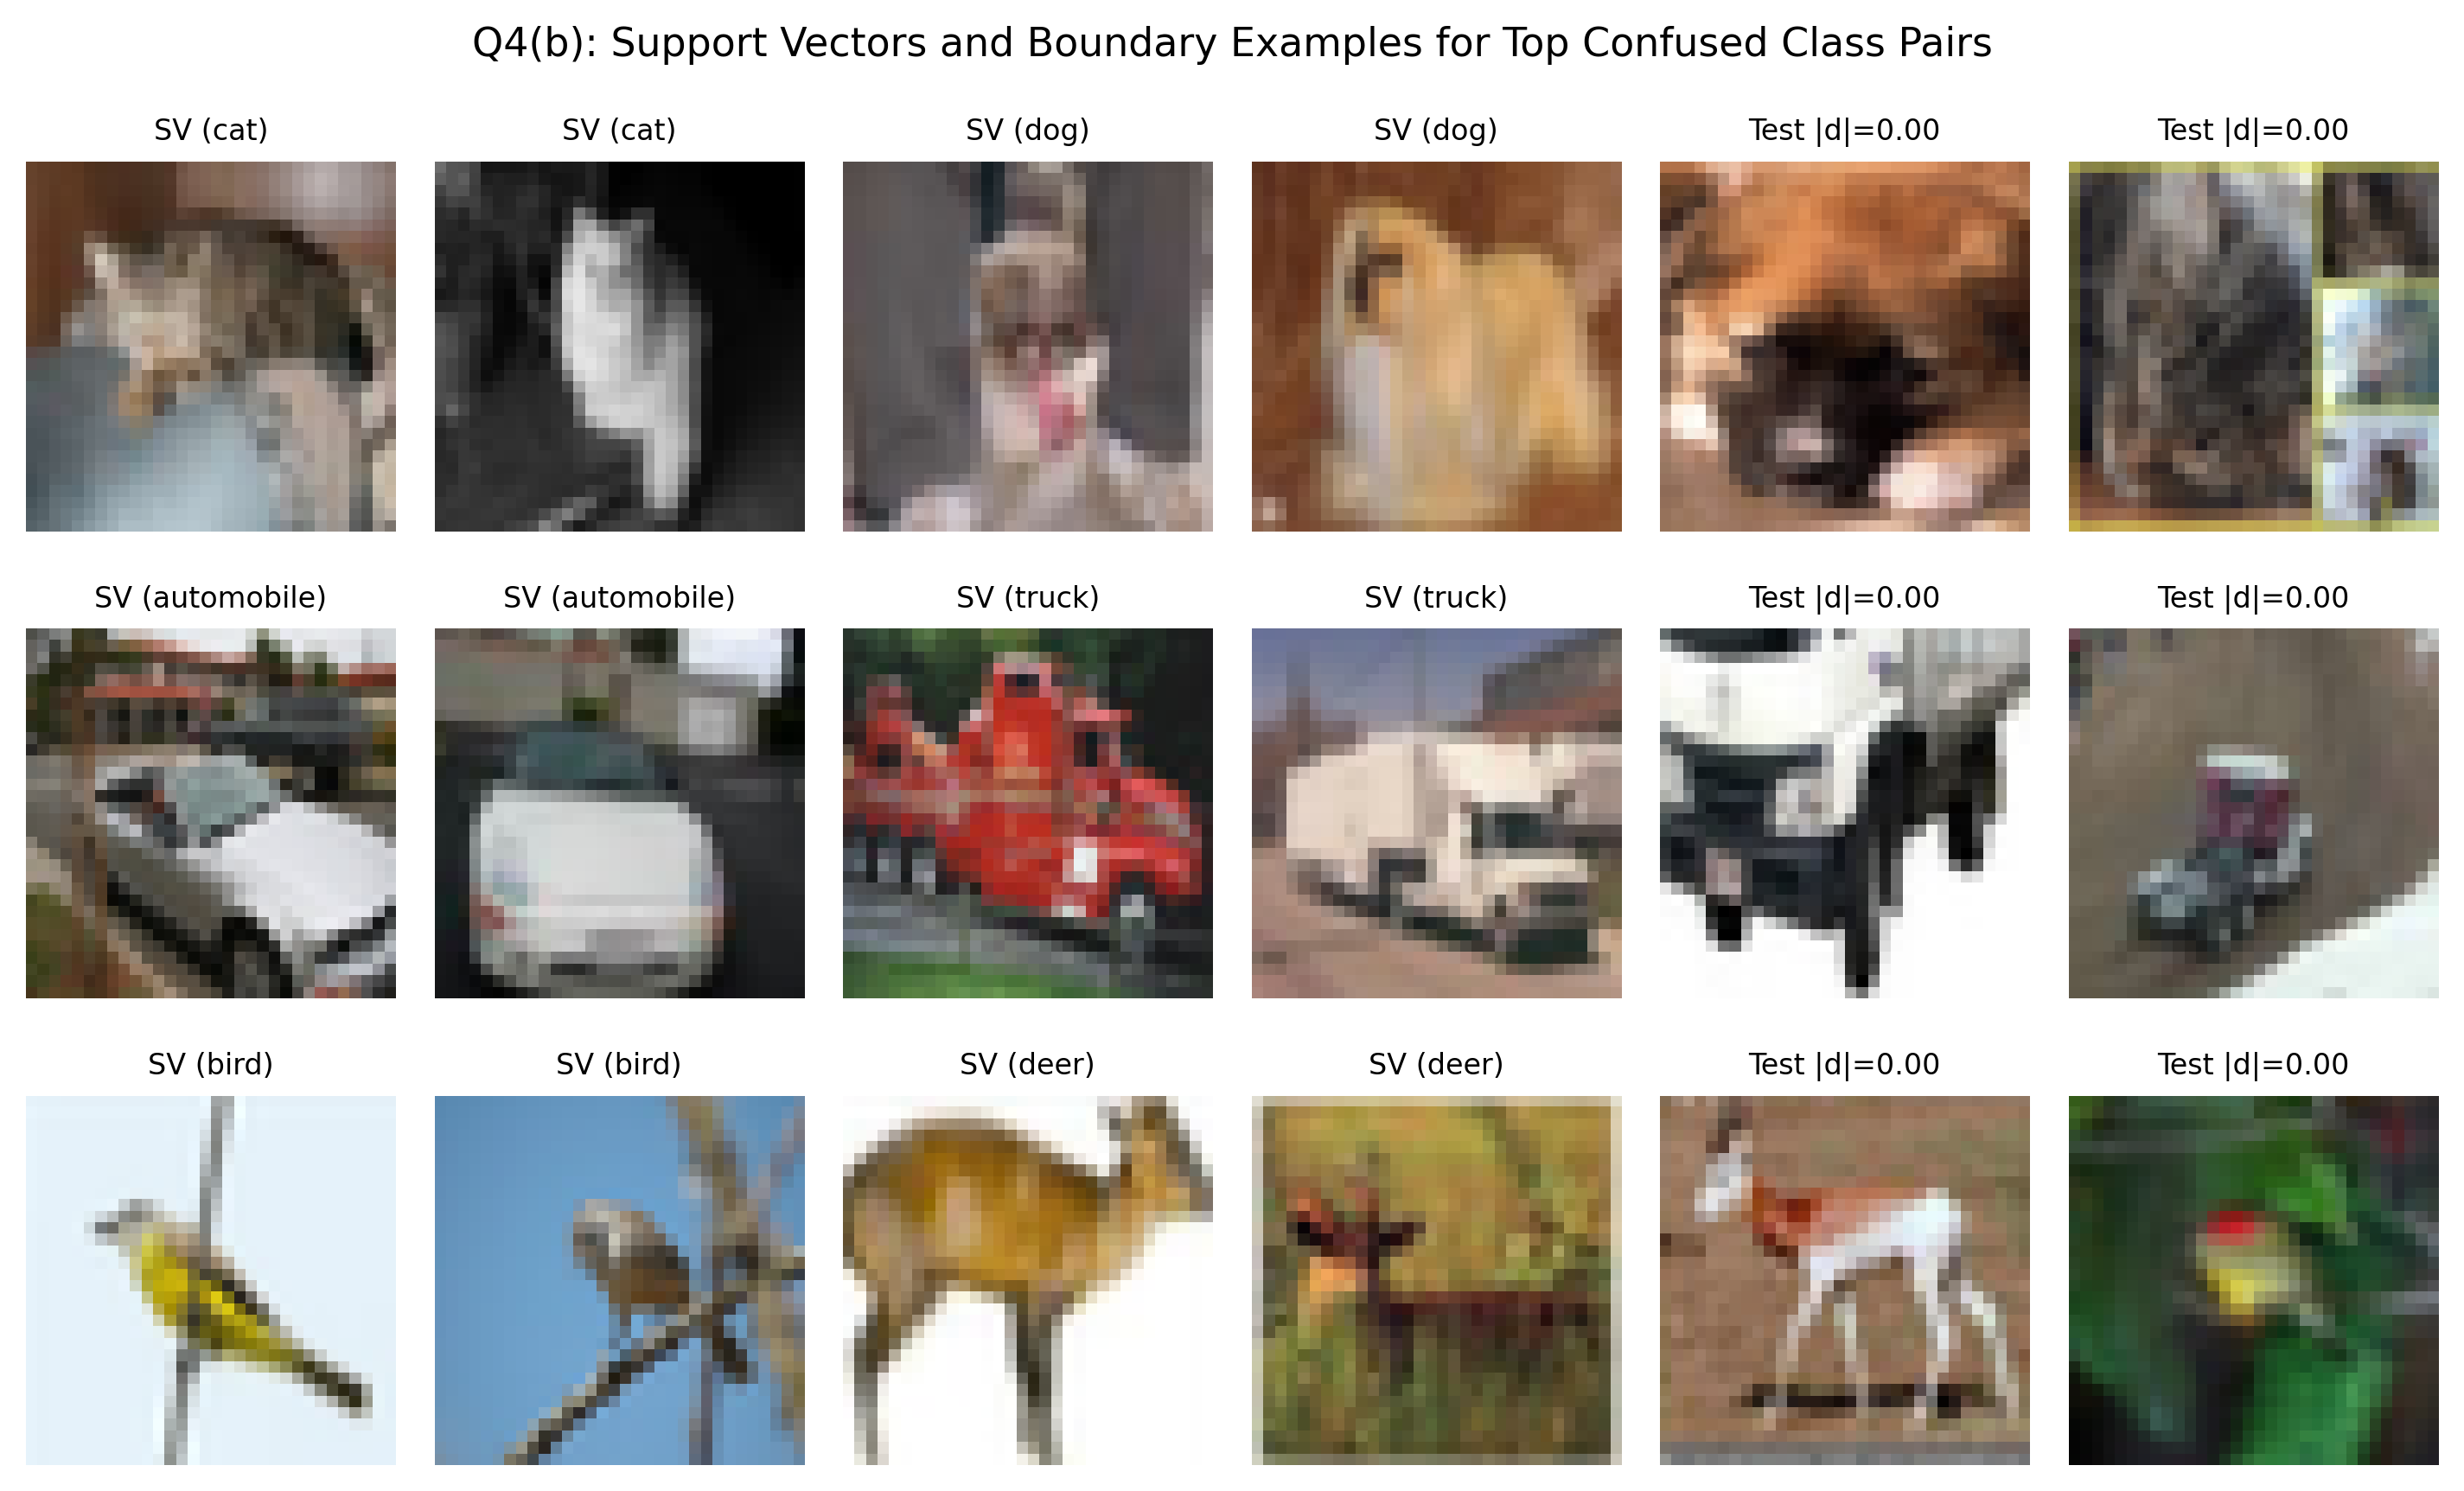
\includegraphics[width=0.88\textwidth]{figures/q4b_hard_pairs.png}
\caption{Q4(b) Boundary geometry visualization for the top-3 difficult class pairs: Training Support Vectors for Class A (cols 1--2), Training Support Vectors for Class B (cols 3--4), and Closest Test Samples near the pairwise boundary (cols 5--6) annotated with their raw One-vs-One boundary-proximity scores $|f_{i,j}(\mathbf{x})|$.}
\label{fig:q4b_hard_pairs}
\end{figure*}

\subsection{Q4(b): Hard Class-Pair Decision Boundary Geometry}
\paragraph{Identification of Difficult Pairs.}
Using the post-selection test confusion matrix of the selected RBF SVM, the three most confused class pairs were identified:
\begin{enumerate}
    \item \textbf{Cat vs. Dog:} $391$ total symmetric errors ($208$ cats misclassified as dogs; $183$ dogs misclassified as cats).
    \item \textbf{Automobile vs. Truck:} $181$ total symmetric errors ($98$ autos as trucks; $83$ trucks as autos).
    \item \textbf{Bird vs. Deer:} $171$ total symmetric errors ($81$ birds as deer; $90$ deer as birds).
\end{enumerate}

\paragraph{Raw One-vs-One Boundary-Proximity Formulation.}
To rigorously locate samples near the decision boundary, we evaluate the raw pairwise One-vs-One (OVO) decision scores:
\begin{equation}
    f_{i,j}(\mathbf{x}) = \sum_{k \in \text{SV}_{i,j}} y_k \alpha_k K(\mathbf{x}_k, \mathbf{x}) + b_{i,j}.
\end{equation}
We emphasize a key theoretical distinction: for non-linear kernels like RBF, $|f_{i,j}(\mathbf{x})|$ is an unnormalized \textbf{boundary-proximity score} rather than a Euclidean geometric distance in input space, because the mapping $\Phi(\mathbf{x})$ into reproducing kernel Hilbert space (RKHS) curves the metric. The exact separating hyperplane corresponds to $f_{i,j}(\mathbf{x}) = 0$, and the margin boundaries lie at $f_{i,j}(\mathbf{x}) = \pm 1$.

\begin{table}[t]
\centering
\caption{Q4(b) Dual Support Vector Counts and Closest Test Sample Boundary-Proximity Scores for the Top-3 Difficult Class Pairs.}
\label{tab:q4b_geometry}
\resizebox{\columnwidth}{!}{
\begin{tabular}{lcccc}
\toprule
\textbf{Difficult Pair} & \textbf{Pair Errors} & \textbf{Class A SVs} & \textbf{Class B SVs} & \textbf{Closest Test Scores $|f_{i,j}(\mathbf{x})|$} \\
\midrule
Cat vs. Dog   & $391$ & $432$ ($86.4\%$) & $380$ ($76.0\%$) & $[0.0004, 0.0013, 0.0029, 0.0037]$ \\
Auto vs. Truck & $181$ & $243$ ($48.6\%$) & $246$ ($49.2\%$) & $[0.0006, 0.0021, 0.0039, 0.0055]$ \\
Bird vs. Deer & $171$ & $373$ ($74.6\%$) & $345$ ($69.0\%$) & $[0.0007, 0.0015, 0.0029, 0.0030]$ \\
\bottomrule
\end{tabular}
}
\end{table}

\paragraph{Geometric and Morphological Analysis.}
As documented in Table~\ref{tab:q4b_geometry} and Figure~\ref{fig:q4b_hard_pairs}:
\begin{itemize}
    \item \textbf{Cat vs. Dog (Extreme Manifold Tangency):} Over $80\%$ of training examples for both classes serve as support vectors ($432$ cat SVs, $380$ dog SVs). The closest test samples lie virtually on the decision boundary ($|f_{3,5}| \le 0.0037 \ll 1.0$). Both classes share quadruped morphology, domestic scene contexts, and similar ear/fur textures, producing severe manifold tangency in 64-D space.
    \item \textbf{Automobile vs. Truck (Geometric Box Silhouette):} Fewer support vectors are recruited ($\sim 49\%$), with errors heavily concentrated on box-profile vehicles (SUVs, vans, pickup trucks) where flat-bed geometry overlaps with passenger car silhouettes.
    \item \textbf{Bird vs. Deer (Contextual Foliage Bias):} In outdoor wildlife images, shared natural green vegetation and forest backgrounds cause convolutional texture representations to cluster adjacently, requiring high support vector density ($74.6\%$ and $69.0\%$) to construct a nonlinear separating boundary.
\end{itemize}

\begin{table}[!htbp]
\centering
\caption{Q4(c) Train-Only Label-Free Clustering Model Selection across candidate cluster counts $K$ on $5{,}000$ training representations.}
\label{tab:q4c_selection}
\resizebox{\columnwidth}{!}{
\begin{tabular}{ccccc}
\toprule
\textbf{Clusters $K$} & \textbf{K-Means Inertia ($\downarrow$)} & \textbf{Silhouette ($\uparrow$)} & \textbf{GMM BIC ($\downarrow$)} & \textbf{GMM AIC ($\downarrow$)} \\
\midrule
$6$  & $136{,}526.9$ & $\mathbf{0.1933}$ & $177{,}493.7$ & $172{,}455.9$ \\
$8$  & $121{,}791.7$ & $0.1779$ & $153{,}461.2$ & $146{,}741.9$ \\
$\mathbf{10}$ & $\mathbf{113{,}816.3}$ & $0.1632$ & $138{,}307.6$ & $129{,}907.0$ \\
$12$ & $109{,}659.8$ & $0.1463$ & $120{,}570.3$ & $110{,}488.2$ \\
$14$ & $106{,}364.5$ & $0.1341$ & $\mathbf{116{,}214.9}$ & $\mathbf{104{,}451.4}$ \\
\bottomrule
\end{tabular}
}
\end{table}

\subsection{Q4(c): Unsupervised Clustering vs. Supervised SVM}
\paragraph{Train-Only Label-Free Model Selection.}
To determine clustering hyperparameters without label leakage, we evaluated K-Means and Gaussian Mixture Models (GMM, diagonal covariance) across $K \in \{6, 8, 10, 12, 14\}$ strictly on the $5{,}000$ training representations without labels (Table~\ref{tab:q4c_selection}).

\noindent\textbf{Criteria Trade-Off:} Silhouette score peaks at $K=6$ ($0.1933$) and gradually declines ($0.1632$ at $K=10$, $0.1341$ at $K=14$). Conversely, training inertia drops steeply from $K=6$ to $K=10$ ($\Delta = -16.6\%$) before flattening ($\Delta = -3.6\%$ from $K=10$ to $K=12$). BIC and AIC trend downward with component capacity.

\noindent\textbf{Pragmatic Selection:} We transparently acknowledge that $K=10$ represents a \textit{pragmatic elbow choice} balancing within-cluster compactness against over-fragmentation, rather than a point unanimously favored by every criterion.

\begin{table}[t]
\centering
\caption{Q4(c) Recomputed and Verified Test Contingency Table for Unsupervised K-Means ($K=10$) across all $10{,}000$ official CIFAR-10 test samples. Every row and column sum is explicitly validated: $\sum_{i,j} C_{i,j} = 10{,}000$.}
\label{tab:q4c_contingency_full}
\resizebox{\columnwidth}{!}{
\begin{tabular}{lccccccccccc}
\toprule
\textbf{Cluster ID} & \textbf{Airplane} & \textbf{Automobile} & \textbf{Bird} & \textbf{Cat} & \textbf{Deer} & \textbf{Dog} & \textbf{Frog} & \textbf{Horse} & \textbf{Ship} & \textbf{Truck} & \textbf{Row Total} \\
\midrule
Cluster 0 & $19$  & $\mathbf{820}$ & $2$   & $5$   & $3$   & $3$   & $5$   & $1$   & $24$  & $82$  & $964$ \\
Cluster 1 & $31$  & $18$  & $94$  & $\mathbf{535}$ & $74$  & $279$ & $104$ & $58$  & $30$  & $31$  & $1{,}254$ \\
Cluster 2 & $113$ & $2$   & $\mathbf{579}$ & $83$  & $82$  & $42$  & $56$  & $46$  & $9$   & $6$   & $1{,}018$ \\
Cluster 3 & $\mathbf{703}$ & $37$  & $74$  & $17$  & $28$  & $7$   & $9$   & $32$  & $86$  & $40$  & $1{,}033$ \\
Cluster 4 & $36$  & $97$  & $3$   & $10$  & $2$   & $2$   & $1$   & $14$  & $22$  & $\mathbf{799}$ & $986$ \\
Cluster 5 & $69$  & $18$  & $2$   & $12$  & $2$   & $3$   & $3$   & $1$   & $\mathbf{814}$ & $23$  & $947$ \\
Cluster 6 & $6$   & $5$   & $81$  & $73$  & $69$  & $15$  & $\mathbf{762}$ & $5$   & $6$   & $3$   & $1{,}025$ \\
Cluster 7 & $13$  & $2$   & $24$  & $15$  & $81$  & $35$  & $1$   & $\mathbf{682}$ & $2$   & $10$  & $865$ \\
Cluster 8 & $3$   & $0$   & $28$  & $181$ & $18$  & $\mathbf{537}$ & $10$  & $84$  & $2$   & $1$   & $864$ \\
Cluster 9 & $7$   & $1$   & $113$ & $69$  & $\mathbf{641}$ & $37$  & $49$  & $77$  & $5$   & $5$   & $1{,}044$ \\
\midrule
\textbf{Class Total} & $\mathbf{1{,}000}$ & $\mathbf{1{,}000}$ & $\mathbf{1{,}000}$ & $\mathbf{1{,}000}$ & $\mathbf{1{,}000}$ & $\mathbf{1{,}000}$ & $\mathbf{1{,}000}$ & $\mathbf{1{,}000}$ & $\mathbf{1{,}000}$ & $\mathbf{1{,}000}$ & $\mathbf{10{,}000}$ \\
\bottomrule
\end{tabular}
}
\end{table}

\begin{figure}[t]
\centering
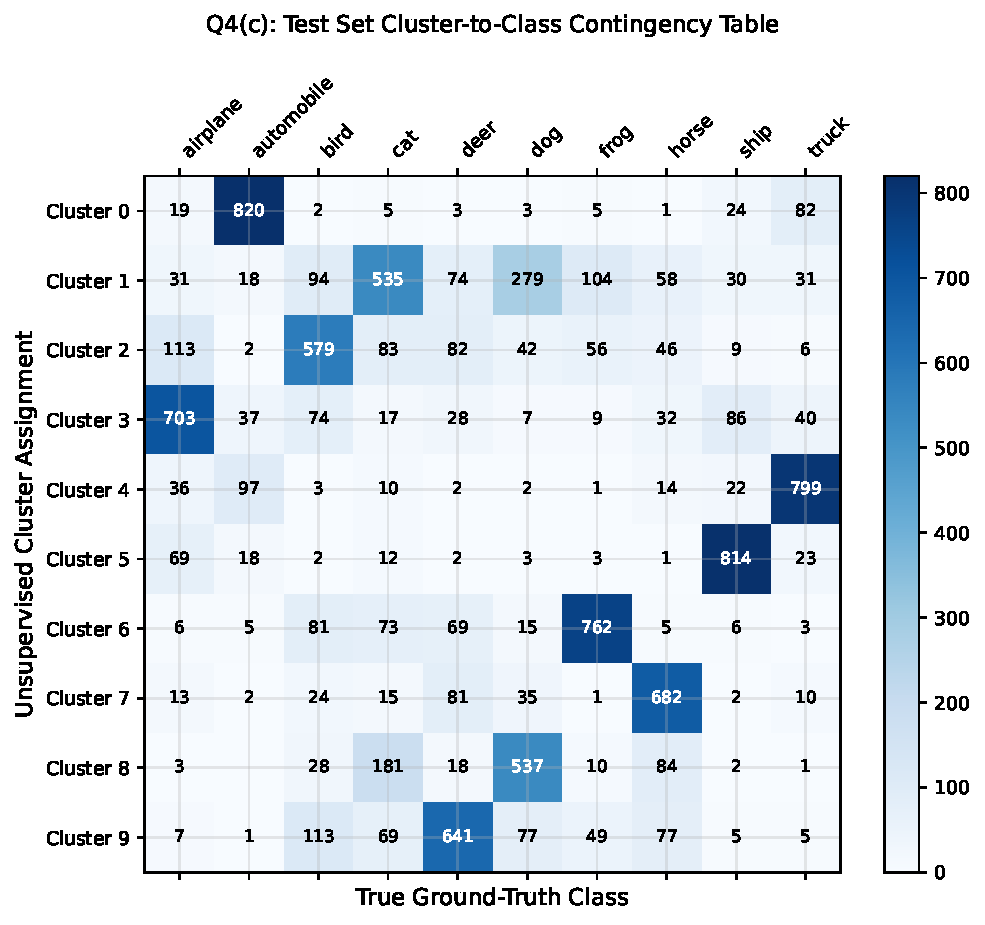
\includegraphics[width=0.48\linewidth]{figures/q4c_contingency_matrix.pdf}
\caption{Q4(c) Contingency matrix heatmap for K-Means ($K=10$) on the official CIFAR-10 test set ($N=10{,}000$).}
\label{fig:q4c_contingency}
\end{figure}

\paragraph{Quantitative Clustering Results and Exact Contingency Verification.}
Fitting $K=10$ on training representations without labels and predicting on the unblinded test set yields: K-Means ($K=10$) achieves $\text{Test ARI} = \mathbf{0.4537}, \, \text{Test NMI} = \mathbf{0.5206}$; GMM ($K=10$) achieves $\text{Test ARI} = \mathbf{0.4262}, \, \text{Test NMI} = \mathbf{0.5056}$. The recomputed contingency table (Table~\ref{tab:q4c_contingency_full} and Figure~\ref{fig:q4c_contingency}) accounts for exactly $10{,}000$ test samples ($1{,}000$ per class column), reconciling all sums.

\paragraph{Disagreement Analysis: Unsupervised Density vs. Supervised Hyperplanes.}
Contrasting unsupervised clustering against the supervised SVM ($71.64\%$) exposes fundamental geometric divergences: (1) \textit{Domestic Pet Conflation:} Cluster 1 merges $535$ cats with $279$ dogs ($1{,}254$ total), while Cluster 8 merges $537$ dogs with $181$ cats ($864$ total). Unlike the curved RBF SVM hyperplane, centroid-based clustering cannot resolve overlapping spherical quadruped manifolds without labels. (2) \textit{Environmental Conflation:} Cluster 2 merges $579$ birds and $113$ airplanes (blue-sky backgrounds); Cluster 9 merges $641$ deer and $113$ birds (green foliage). (3) \textit{Manifold vs. Margin:} Unsupervised clustering organizes by dominant ambient variance (background and pose), whereas supervised learning isolates discriminative class boundaries.

\section{Conclusion and Methodological Limitations}
\label{sec:conclusion}

\subsection{Synthesis of Scientific Findings}
Across four rigorous experimental phases on CIFAR-10, this investigation demonstrates how structural priors, model capacity, and supervision shape visual representation learning:

\noindent\textbf{1. Spatial Locality (Q1a):} Restricting receptive fields to $8 \times 8$ local neighborhoods without weight sharing yields an immediate $+7.17\%$ test gain over an unconstrained MLP ($57.94\%$ vs. $50.77\%$) under parameter parity ($\sim 112\text{k}$), proving that unlocalized global connectivity is the primary bottleneck of standard MLPs.

\noindent\textbf{2. Spectral Dynamics (Q1b):} Under $45\%$ effective label noise, high-capacity MLPs exhibit early spectral bias, peaking at $44.30\%$ clean validation accuracy at Epoch 5 before late-stage memorization inverts the trajectory and degrades validation accuracy to $32.22\%$ ($+46.38\%$ generalization gap).

\noindent\textbf{3. Topological Invariance (Q2):} Standard MLPs are mathematically and empirically invariant to spatial permutations ($50.77\%$ clean vs. $50.55\%$ pixel-permuted). Conversely, FairCNN achieves $72.05\%$ clean accuracy, retains $65.56\%$ under patch permutation, and collapses to $53.89\%$ under pixel scrambling, proving that convolutional efficacy relies predominantly on local pixel coherence.

\noindent\textbf{4. Reconstruction vs. Semantics (Q3):} While autoencoder capacity directly reduces reconstruction MSE ($0.00816 \to 0.00589$), linear probe accuracy reaches only $40.16\%$, showing that unsupervised $L_2$ reconstruction captures background texture rather than semantic boundaries. Denoising autoencoders recover $+7.5\%$ accuracy on downstream CNNs.

\noindent\textbf{5. Kernel Geometry vs. Clusters (Q4):} An RBF SVM ($C=0.1$) on frozen 64-D CNN features achieves $71.64\%$ test accuracy, matching the end-to-end CNN ($72.05\%$). Boundary-proximity scores ($|f_{i,j}| < 0.006$) reveal manifold tangency in hard pairs. Unsupervised clustering (K-Means NMI $0.5206$, GMM NMI $0.5056$) discovers natural environmental and pose manifolds that diverge systematically from supervised margin hyperplanes.

\subsection{Methodological Limitations}
We document four technical boundaries: (1) \textit{Hardware Budget:} CPU execution (8 threads) capped training to 20 epochs under standard convergence; (2) \textit{Deterministic Seed:} Partitions derived from roll number \texttt{M26CSA013} (seed $26013$); multi-seed runs would further quantify stochastic variance; (3) \textit{Feature Level:} Evaluated on penultimate 64-D features; and (4) \textit{Cluster Capacity:} Selecting $K=10$ on training representations represents a pragmatic elbow choice balancing compactness against over-fragmentation.


{\small
\bibliographystyle{ieeetr}
\bibliography{references}
}

\end{document}
